\begin{comment}
Things to get into this section
%===============================

FDA 15	Hotelling / Palander competition dynamics
WUD 16	Hotelling Palander model: simple example for blind agents finding trade-off optima?
Note: this is shorn of all space costs. It's just about the effect of spatial competition. 
WUD 19	Value density: a natural idea from combining utility with Weber-like analysis, and also useful in the real world. Cf. Isard; certain things can be given infinite weight; cf. Storper and trade costs: human-capital intensive = humans are heavy!
WUD 22	Transport intensity: as a concept, need tangled bank?
WUD 22	Externalities, ubiquities, central places, density maps, discrete spatial choices
WUD 22	"CES, supermarkets": explain through love of variety while minimising space/information costs.
%WUD 27	Here and not-here: can be defined with externalities as well as transport costs.
WUD  28-9	Krugman's intermediates. Krugman (and later theorists) are arguing this CES approach to intermediates negates the need for thinking about 'Weber-type problems', and provides a clearer answer.
WUD 31	Such a thing as cost proximity? i.e. distance = further, overall cost = less? Does this mean space can be considered just another factor after all?
WUD 34	What's the difference between a worker and an order of steel? The steel doesn't need to go home and sleep every night. Labour as a factor is unique, and relates to space and time in a particular way. 
Cf.2 migration and commute.
Other random things:
1d vs d2: chapman's intervening opportunities example, and that one paper that looks at the same problem. You know the one! Anyway, they're both in the spacecostswriteup table.
\end{comment}

\chapter{Spatial concepts \label{chapter:spaceconceptsintro}}


%%%%%%%%%%%%%%
% Cutting off for core model writeup
%%%%%%%%%%%%%%
\begin{comment}

\section{Introduction}
%Testing different reference methods. This section reference is without a tilde: section \ref{sec:extsinspace}. This one has a tilde: section~\ref{sec:extsinspace}.

This chapter has three aims:

\begin{itemize}
\item Outline key space concepts
	\item Describe the nature of space costs
	\item Explain what simplifications have been made for the thesis model, and why
\end{itemize}

The concept of space costs covers an unwieldy range of very different dynamics from urban and local to regional and global, with each having its own areas of literature. This is impossible to cover in depth; this chapter picks out those areas that have been used to inform the thesis model-building process. The chapter does this in four sections:

\begin{itemize}
\item Section \ref{sec:spacesituate} gives an overview of spatial economics, picking out the issues of importance for the thesis model.
	\item Section \ref{sec:spacecostgoods} explains how the costs of moving goods and people are defined, and puts them in the context of theories that examine those costs.
	\item Section \ref{sec:extsinspace} looks at the other vital component of space-costs: proximity. The effect  of being `here', and being close to other actors can be in the form of costs or benefits. The theory behind these is discussed.
	\item Section \ref{sec:spacecostissues} is a broader discussion of space costs. Its purpose is to acknowledge the particular complexities of the reality of space costs that have been identified in the literature, and to make an argument for the `strategic simplifications' used in this thesis. The section ends by picking apart the assumptions used to construct the \gls{coremodel} of \gls{ge} as a prelude to chapter \ref{chapter:ABM}.
\end{itemize}

A broad overview is presented of how space costs have been theorised, to give a context for the model choices made. The aim is to find as simple a representation of space costs as possible, within an agent-based framework, without ignoring the aspects of geographical reality useful for the thesis. As the basis of the model is agent-based, there are different simplifications than those prevalent in \gls{ge}. In particular, it is possible to provide actors with simple cost functions that include space, and that each actor must optimise separately. Section \ref{sec:spacecostgoods} explains these. 

There are three particular simplifications that require some justification. First, the use of a featureless Euclidean space. Most of this chapter assumes this space type; section \ref{sec:routedev} explains the reasoning behind doing so and discusses related problems. The second and third most important simplifications are the two opposing forces that the model uses to theorise space costs. These are -

\begin{itemize}
	\item Distance costs: incurred as a result of the physical distance between places. Closer proximity lowers them; further distance increases them.
	\item Density costs: a cost proportional to the density of actors in a given portion of space.
\end{itemize}

Section \ref{sec:spacecostgoods} outlines a very simple approach to costs for moving goods and people that sticks with simple distance. Some of the complicating context of reality is supplied towards the end of the chapter. Density cost is used here as proxy for several types of proximity cost. Section \ref{sec:extsinspace} gives the background for this approach, and section \ref{sec:densitycostsetup} explains its implementation in the model. 

Some space costs are relatively easy to identify; the price paid at petrol pumps is an obvious example, or the time taken to commute to work. Others are less obvious, requiring a theoretical framework to deduce their existence from the data (\citealt{fujita_spatial_2001} p.97). So the chapter ends with section \ref{sec:spacecostissues} by looking at space costs more broadly: what they are, how what is known about them has been deduced, and what theoretical structures are used to analyse them. 

\section{Spatial economics overview \label{sec:spacesituate}}

Spatial economics, both classical and modern, asks the broadest of questions about economic activity: ``who produces what, where and why?'' (\citealt{ohlin_interregional_1933} quoted in \citeauthor{brakman_new_2009}, p.81)  Spatial structure is one of the most obvious facts of economics, and the most difficult to explain. \citeauthor{duranton_micro-foundations_2003} (2003) put it well: ``Only 1.9\% of the land area of the United States was built up or paved by 1992. Yet, despite the wide availability of open space, almost all recent development is less than one kilometre away from earlier development.'' From the point of view of much economic theory, this shouldn't happen at all -

\begin{quote}``If we postulate only the usual list of economic forces, cities should fly apart. The theory of production contains nothing to hold a city together. A city is simply a collection of factors of production, capital, people and land - and land is always far cheaper outside cities than inside. Why don't capital and people move outside, combining themselves with cheaper land and thereby increasing profits?'' (\citealt{lucas_mechanics_1988} , p.38)
\end{quote}

\gls{ge} is the most prominent modern spatial economic theory to offer an answer. Paul Krugman, the original creator of the \gls{coremodel} at the heart of the method, asks, ``why and when does manufacturing become concentrated in a few regions, leaving others relatively undeveloped?'' (\citealt{krugman_increasing_1991}, p.484) The success of \gls{ge} stems from a framework able to address each of Ohlin's `what, where and why'. What is produced? A variety of generic products. The more variety, the better-off the consumers. Where is it produced? There is a `cumulative causation' between the location choice of firms and people, with \gls{increts} as the transmission belt. Combined with transport costs, the core model claims to answer the `why' - a positive feedback flowing from the decisions of rational actors. The model shows how it is possible for one region, with no natural advantage, to end up a core producing area, while another is periphery.

As section \ref{sec:keyconcepts_coremodel} discusses in more depth, \gls{ge}'s approach relies on modelling the interaction between an internalised `iceberg' cost of transport between discrete regions, each internally a point economy, and the effect of externalities for those actors within each region. Distance costs are reduced to a single metric. This contrasts to the Weberian tradition of dealing explicitly with distances and weights for specific firms and goods: this sort of approach is considered good only for `optimal plant location' problems. Krugman only ever mentions `Weber-type stories of transport cost minimisation' to dismiss them (\citealt{krugman_geography_1991} p.49)\footnote{In Fujita, Krugman and Venables' later book (\citeyear{fujita_spatial_2001} p.41) Weber is relegated to a footnote.}. 

This thesis starts from `Weber-type stories': it builds up from distance costs between discrete actors to develop a spatial model and, like both Weber, Isard and \gls{ge}, is interested in the ``general laws'' determining spatial economic outcomes (\citealt{weber_editors_1909} p.xxii). The difference between a Weberian approach and that of \gls{ge} comes down to choice of abstraction. As Fujita notes (\citeyear{fujita_evolution_2010}), Isard, for one, believed that - 

\begin{quote}
``for a balanced treatment, the particular effects of transport and spatial costs in separating producers from each other must be considered. They are too vital to be sidestepped through implicit treatment.'' (\citealt{isard_location_1956} p.26)
\end{quote}

His fundamental reasoning, on the surface, is the same as Krugman's. Isard argued for a `general location theory' to parallel general equilibrium, but railed against general equilibrium's lack of explicit space. For Isard, general equilibrium was a ``wonderland of no dimension'' (ibid). In the period between Isard's and Krugman's work, however, general equilibrium continued to avoid explicit space. As Isserman notes (\citealt{isserman_its_1996}), Krugman repeated Isard's claim almost verbatim, pointing out that ``in the late nineteen-eighties mainsteam economists were almost literally oblivious to the fact that economies aren't dimensionless points in space'' (\citealt{krugman_new_2010}, p.1).  Isard's approach, however, was more Weberian. he argued: 

\begin{quote}
``Since it is the distance factor that is the heart of locational analysis, there is every reason to speak of transport inputs, wherein distance and weight are the two basic factors, and of transport rates as prices of these inputs. Location theorists unfortunately have shied away from such a concept.'' (\citealt{isard_location_1956} p.35)
\end{quote}

Since Isard wrote this, the `distance factor' as he describes it appears to have faded even further. Part of the reason is that Krugman's stated aim in developing his model was to build a bridge between economics and geography, and this meant using key economic elements that rule out a Weberian approach. What was the bait used to lure neoclassical economists out of their dimensionless `wonderland' onto new geographical pastures? A model able to preserve all the key neoclassical features: a self-contained general equilibrium outcome reached through maximising utility, by building on his insights in trade theory that had used \gls{monocomp} to solve the `similar-similar problem' (\citealt{krugman_increasing_2009-1} p.561) of international trade in similar sectors. As section \ref{sec:marketstructure} outlined, the vital element was provided by the new approach to market structure of the Dixit-Stiglitz method: the ability to construct a non-perfect-competition model, required by the neoclassical approach for allowing spatial economic activity to happen at all (see section \ref{sec:marketstructnspace} for more on this).

In doing so, \gls{ge} linked two previously separate outcomes in a general equilibrium framework: geographical morphology and welfare. Actors attempting to find better utility produce specific spatial patterns. This also raised the possibility that welfare can equilibriate while producing radically different spatial outcomes; equally, welfare can change while morphology does not. The success of Krugman's project, however, throws into sharp relief the absence of other attempts to examine these fundamental components of spatial economics. This may be, as Overman notes (quoting Martin \citeyear{martin_new_1999}) that many see -

\begin{quote}
`` - individual optimising behaviour, equilibrium outcomes and mathematical modelling as a regressive step for economic geographers who have `long since abandoned location-theoretic and regional science models'.'' (\citealt{overman_can_2004}, p.505)
\end{quote}

The analytic approach of \gls{ge} is - as many \gls{ge} theorists openly acknowledge - a `mathematical straitjacket' (\citealt{martin_new_1999}). The difference between \gls{ge} and `economic geography proper' (as Martin puts it) is in their evaluation of whether the benefits of the straitjacket outweigh the costs. 

Martin argues that \gls{ge} is unable to properly explain the real internal dynamics that make localisation more productive. Many theorists agree with this while remaining ``squarely on the side of those who consider that general frameworks are necessary to scientific progress in geographic economics'' (Storper 2010 p.315). They want to be able to ``pinpoint the basic sources of urban dynamism, which lie in the selective geographical matching of productive resources, skills and institutions of coordination'' (\citealt{storper_rethinking_2009} p.164). Duranton and Puga have done just that, concentrating on the underlying microfoundational mechanisms of `sharing, matching and learning' taking place (\citealt{duranton_micro-foundations_2003}), as well as broadening out to investigate the ``conditions for a configuration in which diversified and specialized cities co-exist to be a steady state'' (\citealt{duranton_nursery_2001} p.1). See also more recently Delgado \emph{et al.} (\citeyear{delgado_clusters_2010}) for a subtle empirical look at the interaction of clustering, productivity and startups: ``while at a (narrow) industry level firms may compete for the given pool of resources, the cluster environment that surrounds an industry will increase the pool of competitive resources and reduce the barriers of entry for new firms'' (ibid p.514). 
%Storper, however, worries about leaving out the ``wider dynamics that shape the concrete opportunities for and limits on behaviour'' (\citealt{storper_rethinking_2009} p.165).

Some have argued that \gls{abm} is perfectly positioned to help ``bridge the gap between geographical economics and economic geography'' (\citealt{fowler_taking_2007} p.266). As chapter \ref{chapter:ABM} discusses, however, agent modelling seems to have a default affinity with `economic geography proper's outright rejection of everything neoclassical.

The rest of this chapter explains the geographical ideas used in this thesis, as well as the strategic simplifications made.

\subsection{Terminology \label{sec:spaceterms}}

In the thesis model, actors have location in one of two continuous space-types, either a one-dimensional line or a plane. If these spaces wrap, they can be described respectively as a `racetrack' (following Krugman) or a torus. In the rest of the thesis, these types of space will be labelled $R^1$ or $R^2$. $R^1$ is just the real number line $R$, but using $R^1$ indicates that a one-dimensional space is being discussed. Strictly speaking, neither of these are accurate for describing a one-dimensional racetrack or two-dimensional torus, but it is a useful shorthand. 

The implications of these types is discussed below, but from the point of view of the thesis models, the differences between them boils down to how actors' location choices are restricted. All other model features remain the same. (This also means that discrete spaces can be `simulated' by simply restricting actors to binary location choices.)

Some very basic differences exist between $R^1$ and $R^2$ when costs are changed. Most simply, whereas in $R^1$, a doubling of distance leads to a doubling of space covered, in $R^2$, the area covered is quadrupled ($\pi(2r)^2$ is $\pi 4r^2$). If, for example, potential economic actors are evenly spread across space, there is thus a four-fold difference in the number of new interactions the doubling enables.

Most of the analysis uses forms of continuous space. A quick note on monocentric models is in order, however. A monocentric model, as the name suggests, has a set point around which economic activity is analysed, both in $R^1$ and $R^2$. As Fujita \emph{et al.} note the von-Thunen style model, reformulated by Alonso into the classic monocentric model of urban economics, is limited because ``if your question is not simply how land use is determined when the location of the town or towns - indeed their number and size - is itself endogenous - the von Thunen model offers no help'' (\citealt{fujita_spatial_2001} p.18). For the thesis models, however, it quickly transpired that fixing a monocentric point was a very effective method for testing how different space costs interact. Section \ref{sec:spatialeq} thus uses a number of `monocentric' style models.

Space costs can be theorised as having three components, separate from whatever is being moved across space:

\begin{enumerate}
	\item \Gls{mbf}: actors must `spend' these to get themselves and goods across any distance. Time can be an \gls{mbf}; others are discussed below.
	\item Technology: this changes the level of \gls{mbf}s required to `buy' a given unit of distance.
	\item Infrastructure: development, such as road and rail networks or ports, that affect both technology and \gls{mbf}s.
\end{enumerate}}

The cost of moving people and of moving goods can be described using different \gls{mbf}s. People must incur a time-cost: this is their primary \gls{mbf}. In reality, more than one will be spent to get across space. Note that, in the thesis model, actors do \emph{not} need to `buy' migration. That is, if an actor moves their permanent location, this is free. It costs them to move goods or move themselves to a workplace; see section \ref{sec:peoplemoving} for more detail.

Infrastructure, it will be argued, is beyond the scope of this thesis to consider but, as in \gls{ge}, it is a reality that needs to be consciously and carefully placed outside the analysis. This is done in section \ref{sec:routedev}. 

Each of these is associated with a particular timescale in which change affects actor decisions, and changes within one feeds into to the others. \gls{mbf}s are the most short-term consideration. For instance, if fuel prices change, actors will immediately alter their behaviour - though fuel is a particularly inelastic commodity, so the changes will be slight. Technology change is more medium term. Using the same example, technological responses to fuel cost change have been clearly identified: actors alter technology choices in the medium-run by changing car. On the supply side, companies respond to those fuel costs by building more efficient vehicles. Short-run and long-run elasticities for fuel costs, then, are reflected immediately in how much movement actors will `buy', and then in their choice of mode and vehicle. Technological change can also open up entirely new trade doorways: for example, refrigeration for meat opened up new export markets for Argentina and New Zealand (\citealt{chapman_people_1979} p.182). In the longer-run, larger-scale technology changes blend into infrastructure development as the two co-develop. 

\section{Cost of moving goods and people \label{sec:spacecostgoods}}

Analysing the reality of moving goods and people across space is beset by the many idiosyncracies both of these have. A particular approach has been developed for the thesis model that tries to simplify these costs into a coherent set of factors. The following sections lay out this approach, while also discussing some of the more thorny issues real-world space costs have.

The full cost of moving goods and people goes beyond simple considerations of distance. Section \ref{sec:spacecostissues} looks at some of these considerations to give some context. The models developed for the thesis, however, do stick to examining how actors interact given simple space costs affected by distance or density. 
%Fujita et al.: ``There are two main sources of evidence on this question. The first is to try to measure these costs directly, and the second comes from looking at trade volumes, and seeing how rapidly they fall off over distance'' (\citealt{fujita_spatial_2001} p.97).

Section \ref{sec:spatialeq} compares the effect of changing a series of space costs and, as discussed in detail there, the modelling process revealed parallels between changing good- and people-moving costs. In short, the non-spatial part of cost changes (such as the base price of goods before delivery costs, or the wage itself, without costs related to commuting) have an opposite effect to the spatial parts. This section sets the scene for the later models by describing how, while on the surface the costs associated with moving people and goods are structurally quite different, they nevertheless have similar effects. 
%Rubbish para! Ah well.

%Section \ref{sec:factors1} - explaining about exchange of factors being at the heart of economics, and spatial economics. 
Section \ref{sec:factors1} introduced the idea of factors and how they are used in the model. The approach to time as a factor is quite specific and needs some explanation. `Time as a factor' can only be used to do two things: `buy' movement or pay for other factors (either output or money). Decisions using `time as a factor' happen in one model iteration, not over several as would be the case with many real-world time-based economic activities. 

This is potentially confusing: time is a factor used in each model iteration, but it is completely distinct from a common understanding of time-based decisions spread over shorter or longer timespans. So why use the idea of time at all? It is certainly a massive simplification to treat it as `just another factor', exchangeable for other factors. For example, in reality, real-world freight shipment happens over many days, weeks and even months and can be modelled accordingly (see, for example, \citealt{hummels_time_2001}). It also underpins problems of risk and uncertainty in trade across space (see section \ref{sec:spacerisk}). 

There are two reasons it is worth thinking about time. The first is the primacy of time for the decisions people take about space - for example, the relationship between home location and commuting times. The second is that time is unique, in that an uninterrupted flow is given freely to actors, at exactly the same constant rate. It is exogenous to production and space. Equally, once used - either `spent' on space or production - it `melts away'. Most of the models presented here do give actors a constant `fixed income' in this way; this can equally be considered as a fixed daily income or a `free gift' flow of time to optimise. If there is an intermediary stage of acquiring a wage, it still needs to be bought with labour, which then reduces back to time again. Time can thus become, if not the numeraire (see section \ref{sec:comm_costs}), then certainly a practical base for comparison.

The rest of this section explains the way space costs are defined for goods and people.

%"The point is - what happens when they change?"
%Yes! That is the point! Brilliant. And of course, this separation of base and space cost as regards how actors react to density cost is perfect for that. But not very good for the larger picture, where we probably have to think about fixed positions.

\subsection{Cost of moving goods \label{sec:costmovinggoods}}

%%\subsubsection{How good movement works in the thesis models}

A simple mathemathical way to describe the cost of moving goods across space is as follows. Let $P_g$ be the full cost of one unit of good $g$, $p_g$ the base per unit cost, before any space-costs; $c$ the cost to move one unit of this good over one unit of space, and $d$ the distance moved. Then - 

\begin{equation}
P_g = p_g + (c\cdot d)
\label{eq:spacecost}
\end{equation}

On a given model iteration, this will be the cost faced by actors wanting to buy the goods. In line with the simple approach to time, no distance will be too large for goods to travel during one iteration, but the total cost, including $cd$, may be too high. 

$c$ represents a catch-all variable for the generic costs of moving goods, whether due to weight, bulk or some other factor. (It could also be defined to include other factors that produce \gls{increts} to distance; that is, the further a unit is moved, the cheaper per unit of distance it becomes, as variable delivery costs increase relative to fixed delivery costs.) For the purpose of this section, the important point is to note the impact of varying $p_g$, $c$ and $d$. 

One way of thinking about this effect is to use the idea of `value density'. This can be defined as the ratio of product value to physical size or weight (\citealt{lovell_product_2005} p.144); here, that is $p/c$, with $c$ standing in as a proxy for generic per-unit shipping cost. What this idea shows is that, the more value is added, the more feasible large space costs become. That is, if $p$ is increased, the good does become more expensive - but space becomes relatively less important. Conversely, as Lovell \emph{et al.} note, ``as the value density of a product decreases the percentage of additional distribution costs increases.'' (ibid.)

More value is added, by definition, with larger \gls{increts} (see section \ref{sec:prodfuncts}). A unit of input labour can produce a higher output. That output, however, could be measured either in added value or an increase in physical output. This is an old point of Weber's: he distinguished between processing that added weight or removed it. In equation \eqref{eq:spacecost} above, the addition or subtraction of weight would be reflected in $c$, and changes in value in $p$. Lovell \emph{et al.} note Coopers' research on the production of microchips as a classic example of combining massive scale with very high value density (\citealt{cooper_logistics_1990} in \citealt{lovell_product_2005} p.144). Glaeser and Kohlhase give a good list of shipped goods with different value densities: in the U.S., wood products' average shipment length was 287 miles at their time of writing and transport costs a fifth of the value. For base metal, a tenth of the value went on transport. In contrast, machinery and electrical goods were always less than 1.2\% transport costs (\citealt{glaeser_cities_2004} p.208).

As section \ref{sec:routedev} explains, choice of transport mode is excluded from the model, but it is worth noting the relationship between value density and mode choice. As Lovell points out, it is only high value-density goods that get air-freighted (\citealt{lovell_product_2005} p.153). This highlights how important, in reality, the time element of good transport is. 

%[207] According to their analysis: only 18\% of all shipments occur in industries where transport costs are more than 6\% of total value - even if all transport was by truck."  Q: how is JIT affected by mode choice? [23]

%---

Equation \eqref{eq:spacecost} takes a very literal approach to distance, in contrast to the `iceberg' transport costs of the \gls{coremodel}, where the goods themselves `melt away' and a single parameter controls ``the number of goods that need to be shipped to ensure that one unit of a variety of manufactures arrives per unit of distance'' (\citealt{brakman_new_2009} p.109). In \gls{ge}, distance is used as a broader term that can include general trade-cost impediments to the exchange of goods across space. For an \gls{abm} approach, it makes sense to treat distance in the more literal way done here, as actors face making decisions about specific goods with given prices.
%Distance itself: if 2, Trs = 4... see WUD `On space costs'.


\subsection{Cost of moving people \label{sec:peoplemoving}}

There is a hard limit to people's time: a flow of twenty-four hours per day must be spent. Because of this, one way to model distance for people in the model is to build up from the idea of one `day' and the distance people can get in that day. This approach is as follows: 

\begin{itemize}
%\item For each model day, each actor is given $t=1$ to spend: in other words, they have `one day per day' and will aim to make optimum use of it. (See note below for more on this.)
\item For a given distance $d$, the time is takes to cover it is $t_{d}$. So, generically, $t_{d}=f(d,tech)$, where $tech$ is some technology that has an impact on the time taken. For many of the models, time to cover a given distance will be a function of the distance alone. However, the generic factor $tech$ here indicates that the amount of time to cover a distance may change. 
\item $tech$'s role in this function is separate from its cost. For example, if $t_{d}=d/tech$, the time taken to travel $d$ goes down as the level of $tech$ increases. It says nothing about $tech$'s cost. Indeed, from the point of view of actors, it could be free and ubiquitous.
\end{itemize}

The spatial consequences of this are most strongly felt for those activities requiring the most time - and employment tops this list. Close seconds are access to housing and goods. The spatial solution to this problem does not necessarily require people to stay within a day's radius: Ojo, for example, studied agricultural `commuters' in 1970s Yorubaland who developed a ``fortnightly pattern of periodic commuting to reduce the friction of distance'', moving between more distant settlements (\citealt{ojo_journey_1973} p.86; \citealt{chapman_people_1979} p.122). Closer to home, commute patterns that span larger distances than one day's range are not uncommon, but the vast majority keep to the geographical limit bounded by feasible daily commute times.

The cost of moving people is of paramount importance to firms; the idea of external costs comes in particularly useful here. Firms face these costs from people travelling to work or moving to get goods and services. Firms primarily want to locate near to labour: as well as being intuitively obvious, this is a key finding from the literature. For instance, ``using the same workers is approximately eight times more likely to increase the degree of co-location than are trade relationships'' (\citealt{glaeser_cities_2004} p.223).  Similarly, service providers are usually reliant on proximity to customers. In both cases, the same \emph{type} of space cost exists: that incurred by people moving location. A simple example would be a hairdresser: the service provider has externalised one of the major costs - getting the person's head under the scissors from some distance away. In the case of commuting, the cost is less cleanly external or internal to the firm's production structure, since wages in part must cover it. (Section \ref{sec:firmsLoV} has an example of such an external cost and how two firms cope with them.)

For people, the direct financial cost of transport is very high, relative to how much it costs firms to move goods. Button finds that ``after housing and food, transport represents, at about 10 to 15 percent for a single-car-owning household, the largest element of expenditure out of income in industrialised countries'' (\citealt{button_transport_2010} p.90). In the U.S., Glaeser and Kohlhase note both the money and non-money movement costs people face: they cite a 2001 consumer expenditure survey showing that, in the U.S., ``18\% of total expenditures for the average household is spent on vehicle purchases, gasoline and other vehicular expenses'' - but point out that time costs are not accounted for in that, and that ``these time costs are not withering away with technological progress'' (\citealt{glaeser_cities_2004} p.208). 
%tie to theory of people as productive units.

People's time has become increasingly the most important space cost. This is an argument made most forcibly by Glaeser (\citealt{ glaeser_cities_2004}, \citealt{ glaeser_cities_2008}; see also \citealt{beckmann_lectures_2010}, p.3). The reason is intuitive enough: as transport costs for goods drop, time becomes relatively more important. A knock-on consequence has been to emphasise those elements of human productivity that rely on time proximity. Leamer and Storper explain this by pointing out that -

\begin{quote}
``humans remain the containers for shipping complex uncodifiable information. The time costs of shipping these containers is on the rise because of congestion on the roads and in the airports while the financial costs of so doing are also rising due to increases in real wages of knowledge workers who are the human containers'' (\citealt{leamer_economy_2001} p.648).  
\end{quote}

The precise nature of these human time-proximity effects are harder to pin down; see the discussion of localisation externalities below. 

\subsection{Reframing the cost of moving people \label{sec:reframingpeoplecost}}

Section \ref{sec:wageselect} outlines in detail one approach to how people's time can determine their wage. Simply, the amount of time remaining to contribute to an employer will be less if a person is further away. If an employer pays a given wage for a unit of time contributed, at $d=0$, the person gets a full unit of wage. At the one day limit, however, they will get no wage at all. (This is, of course, another unrealistic approach: see below for further discussion on this.) The model can be set up so that people select employers on this basis. However, as section \ref{sec:spatialeq} will later explain, it is useful to understand the parallel between good movement and people movement when it comes to describing their effect on spatial outcomes. 

In the situation just described, if a firm was paying a wage of $w=1$ and $tech=1$, the person's wage will just be $w=t-d$, with the imposed condition that if $d$ is over the hard time limit, the person cannot consider that firm as an employer. This is easy enough to code but not a very satisfactory analytic approach. It also masks the difference between the non-spatial and spatial elements by subsuming them in one function.

It can be reframed in a way that parallels the description of good costs used in section \ref{sec:costmovinggoods} above. To do this, the cost element needs to be separated from the budget element, as follows. A firm is not offering a wage: rather, they are selling a factor - in this case, money - in precisely the same way they sell goods at a given price. (This will also come in useful later when actors are exchanging factors other than money.) The amount supplied is just $g=f/p_g$, where $g$ is the supplied factor, $f$ is the payment and $p_g$ the price of $g$. 

In these terms, people are just buying money with time. The price a firm will charge is as just stated: $p_g$ for one unit of money. What about the space cost element? The uniqueness of moving people, it has been claimed, is the hard limit to time, beyond which no wage can be bought. The good-cost function above would not do this job: regardless of how high the price goes, some small quantity is always demanded. The only way such a hard limit could work is if the cost of money becomes infinite at the hard limit. This can be done as follows, using the variable definitions already given above. At the point where $d/tech = 1$, $p_g$ is divided by zero and the cost becomes infinite:

\begin{equation}
P_g = \frac{p_g}{1 - (d/tech)}\label{eq:wagespacecost}
\end{equation}

A person with a time-budget of $t=1$ must optimise given these costs. Assuming they are only `buying money' from one firm (an assumption changed later) , they will want to spend their whole budget on the single cheapest supply. The amount they can buy in this situation is just their budget divided by the full price described in \eqref{eq:wagespacecost}. Assume $t$ and $tech$ equal one, then the amount they can buy is just their time divided by the price:

\begin{equation}
g = \frac{t}{p_g/(1-d)}\ = \frac{(1-d)t}{p_g}
\end{equation}

This brings the description full circle: if the `price of money' is one, the amount the person gets is proportional to what is left after distance has been accounted for. 

What was the point of this long roundabout trip? Three things: firstly, to highlight that the more algorithmic description of people getting their wage can be reframed into a simple optimisation problem with a price and a budget. Secondly, to illustrate that different cost functions can be made to achieve particular spatial outcomes. Section \ref{sec:prodtowelfare} will discuss this further, in a model where people are paid directly in goods using the less hard-cutoff cost equation \eqref{eq:spacecost} above. Lastly, as mentioned, this allows the clear separation of the `cost of money' and the space cost involved, which here is controlled by $tech$. Section \ref{sec:spatialeq} will use this to compare the effects of spatial versus non-spatial cost change. 


%"there's no way that a wage change can do anything to alter the hard time limit"
%Only a tech change can do that
%I've set it up currently so the cost of money is defined in terms of time: People pay for money with time.

\subsection{The interaction of people and goods \label{}}

The most obvious difference between moving people and goods is the distance they cover. The prominence of time-cost for people dominates. (As mentioned, while time is a key cost for moving goods in reality, here the time element of good movement is ignored.) Good movement also does not impose the same hard limit: distance means smaller demand, but not necessarily zero demand. The geographical result of these differences is an economic landscape adapted to minimise both people-costs and good-costs into a series of overlapping plates of economic activity. As Isard put it:

\begin{quote}
``Each individual commodity market including its labour, capital and land orientation possesses a particular structure which offers a certain resistance to change. Some change frequently, others slowly. Some are active, others highly inactive. By definition those markets of a relatively permanent nature, of persistent inactivity, are grouped together as the essential ones... Their combined structure determines the basic structure of the Gestalt whole, of the space economy under question.'' (\citealt{isard_location_1956} p.39)
\end{quote}

This goes back to the problem of analysing the complete impact of costs, not just those that can be measured - a point made by Burstein \emph{et al.}, who note that concentrating just on incurred costs is - 

\begin{quote}
`` - likely to underestimate true transportation costs. This is because we do not observe the cases in which transportation costs were so high that the transaction did not take place.'' (\citealt{burstein_distribution_2003} p.1198)
\end{quote}

While this problem is easy to state, it is harder to work out how those costs could be quantified. After all, it is essentially a counterfactual: what trades would have taken place if costs were lower or demand higher? The fact remains, however, that the observable situation is one where cost minimisation has already taken place. There is an overlap here with the idea of `demand thresholds', where high costs cut off transactions (\citealt{chapman_people_1979} p.86).  This has tended to be applied to consumer demand problems, rather than the economy as a whole. It is certainly easiest to understand Burstein's point by applying it to people: as discussed above, time thresholds mark a clear limit on how far people can travel to work (without needing some strategy to get around the day's time limit). The same applies to firm inputs other than labour, however. Value density and demand combine to limit the feasible range any good can be traded. One possible solution is to compare the difference that cost changes make in a model; this is done in section \ref{sec:testspace}.

The size of the ratio of space costs to other costs is an important determinant for actor outcomes. Consider the service industry: Glaeser and Kohlhase correctly point out that since ``transportation costs for people are still high, but transportation costs for goods are not'' (\citealt{glaeser_cities_2004} p.220), proximity to people is the most important spatial factor for services. They also note (p.201) that ``services tend to involve little freight shipment''. But what about transport costs as a proportion of the service sectors' overall costs? For the U.K. at least, Diamond and Spence found they were 9.9\%, compared to 4.7\% in manufacturing (\citealt{diamond_infrastructure_1989} in \citealt{button_transport_2010} p.58). Unsurprisingly, much of the service sector has lower overheads than other sectors. The paradoxical result is that services are more space cost sensitive. 

%This important argument is returned to in the concluding discussion in section \ref{sec:ecocrit}, but to end on some key points:
%Glaeser argues that transport costs are so low that they need not be considered in analyses: only people's time costs are worth paying attention to. 

The introduction began with Glaeser and Kolhase claiming that ``it is better to assume that moving goods is essentially costless than to assume that moving goods is an important component of the production process'' (\citealt{glaeser_cities_2004}, p.199). They are certainly right about the relative change in importance for time versus other space costs, but assuming away those other space costs is a large step to take. 

This point overlaps with the `ecological criticism' discussed in section \ref{sec:ecocrit}: it seems, mathematically, that the importance of transport costs can be reduced simply by \emp{increasing} the cost of other inputs into the production process. By making other inputs more valuable, the importance of space can be lessened, with no limit on how much they can be reduced. 

A spatial version of the ecological criticism might go like this: it is obviously nonsense to think that distance costs can be reduced to nearly zero simply by increasing the value of other inputs. First, there are hard cost limits to moving goods and people. Second, economic value cannot be magically conjured out of thin air; as Daly put it, one cannot simply `stir faster in a bigger bowl'. Space is a crucial ingredient. Exactly how little of that ingredient is required? This problem is central to recent attempts to find ways of `decoupling' transport and economic productivity. Decoupling can be defined as ``achieving economic development without a proportional increase in transport activity (and emissions)" (\citealt{gray_decoupling_2006} p.3). Historically these two have been umbilically linked (\citealt{echenique_separating_2002}) and, while there is evidence that transport intensity (amount of transport per unit of GDP) has been dropping in the richest countries, an attendant increase in demand for oil in developing countries suggests that outsourcing of high-intensity activities is at least partly responsible (\citealt{roberts_oil_2010} p.29). 

As chapter \ref{chapter:ABM} discusses, there are no easy routes to dismissing Glaeser's simplifying assumptions out of hand as ``unacceptably distorted'' (\citealt{granovetter_sociology_2001} p.9). But ruling out non-time space costs in this way appears to also rule out asking, `what happens when they change?' It also makes it difficult, if not impossible, to investigate the relationship between space costs and productivity. 


%Now, the example of the service industry suggests that the less transport costs are part of a firm's production function, the less their decisions will be determined by spatial considerations. More broadly, value density indicates the same things for goods moving within firm production networks, and on to consumers. But Glaeser's argument is clearly not that space has stopped mattering. 
%The question seems to be: what happens in space when good costs and people costs change, relative to each other? The thesis model is set up to examine this problem.
%A world where space no longer matters is science fiction. Indeed, Chapman imagines something like that, where Star Trek's teleporters are the norm: "the universal availability of the kind of technology at the disposal of the Star-trekkers would transform these [spatial] relationships by effectively nullifying the role of distance as an obstacle to movement between one place and another." (\citealt{chapman})

\section{The costs and benefits of proximity \label{sec:extsinspace}}
\subsection{Externalities versus proximity \label{sec:externalitiesspace}}

The obvious benefit of proximity is a simple cost saving: being nearer means less distance to cover. This is a point often absent from discussions of space costs. Black and Henderson (\citeyear{black_spatial_1999}, p.327) are one of the few to explicitly mention it: ``capital good plants agglomerate in locations with high manufacturing employment even though this generates no externalities: it just conserves on transport costs of exchange.'' More usually, the costs and benefits of proximity are described using the language of externalities. (This issue is discussed in more depth below, using the \gls{coremodel} as an example.)

A localisation externality\footnote{The terminology used varies widely and can be confusing. These are agglomeration effects (sometimes described in the literature as `localisation externalities' or `localisation economies'; e.g. \citealt{malmberg_elusive_2002}, \citealt{wheeler_localization_2007}, \citealt{figueiredo_localization_2009}). Glaeser talks of `agglomeration economies' that ``exist whenever people become more productive through proximity to others'' (\citealt{glaeser_cities_2008} p.5). Again, by the definition used here, these are agglomeration effects.  There are many different terms for the opposite of agglomeration: classically, Weber used `deglomeration' (\citealt{weber_theory_1909}); Krugman uses centrifugal forces, opposed to centripetal forces holding places together; Brakman \emph{et al.} (\citeayear{brakman_new_2009}) use `spreading'. This thesis will use dispersion, following Fujita and Thisse (\citeyear{fujita_agglomeration_2002}).} 
is an effect that derives from being `here', and can be either a cost or benefit. In much of the literature, `here' is a discrete place, which actors are either inside or out. Section \ref{sec:externalities} explained that externalities can be defined by introducing external values directly into an actors' utility or production function, or introducing them after these - for example, into a firm's income level. In a discrete space, external economies are easily implemented. For instance, in a two-region model with regions $r$ and $s$, firms in $r$ could include in their production function the total output of other firms in that region, $nx$. Using Scitovsky's way of defining an externality, that would be:

\begin{equation}
x_{r}=F(l_{1},c_{1},...;nx)\label{eq:locext1}
\end{equation}

In Scitovsky's terms, this is a pure externality since it enters directly into the production function. Economically, what does it mean? The classic example goes back to Marshall: the number of firms of the same industry in one locality increases the stock of knowledge for all firms there. This can be explained in terms of the number of workers in a region also; their presence acts as a knowledge multiplier as they move between firms. (See e.g. \citealt{ krugman_geography_1991} pp.36, and Marshall himself, \citeyear{ marshall_principles_1895} pp.349.)

These `Marshall externalities' are often contrasted to `Jacobs externalities'. These attempt to capture the central thrust of Jane Jacobs' argument: that diversity of production lies at the heart of regional productivity (\citealt{jacobs_economy_1970}, \citeyear{jacobs_cities_1986}). A simple way of achieving this would be to insert a CES-type function into \ref{eq:locext1} rather than the raw number of firms: a region's productivity could thus, in effect, have a `love of variety'. Duranton and Puga (\citeyear{duranton_micro-foundations_2003} pp.4) use a more sophisticated version of this to model a region's gain from sharing a variety of intermediate inputs. The effect of competition between firms can also be reduced to an externality in the same way: this is a key feature of the \gls{coremodel} (see section \ref{sec:keyconcepts_coremodel} for more details.)

The common element to all localisation externalities is mathematically describing a relation to help explain the effect of many actors being in close proximity. Doing this for discrete regions (as, for instance, the \gls{coremodel} does) has clear advantages. The effect of proximity is definable in a tidy way. One of the clearest benefits of this is empirical comparability. Being able to define a direct mathematical relationship between regional output or diversity and overall firm levels gives a simple route to regression analysis - a fact used by Glaeser \emph{et al.} (\citeyear{glaeser_growth_1992}) to identify Jacobs externalities as the most powerful (a result since challenged by \citealt{van_der_panne_agglomeration_2004}). 

A central theme examined in chapter \ref{chapter:ABM} is knowing what level of analysis is under examination, and this point is vital for discussing externalities in space. Localisation externalities can be seen as `black box' proxies for describing aggregate economic effects, supported by an argument about the market structure that underpins it. 

As the next section explains, this thesis uses a `second nature' proxy, a `density cost'. As the same suggests, its effects are not based on a discrete absence or presence of other economic actors. The rest of this section looks at the ideas used to argue for a density cost approach. 

\subsection{Land cost and congestion \label{sec:landcostcong}}

The thesis model uses density cost as a proxy for both land costs and congestion. It is not intuitively obvious that these two can be lumped together; this section explains the argument behind doing so.

Space has two fundamental kinds of cost. The first comes from distance; this has been the subject of most of this chapter so far.  Distance itself is not the cost, but rather it forces actors to spend \gls{mbf}s to traverse it. It is this space that Weber worked with (\citealt{ weber_theory_1909}): for instance, the Weber-Fermat problem (see e.g. \citealt{brimberg_fermat-weber_1995}) of optimising a plant location given two inputs and a market happens on an otherwise entirely featureless and costless surface, and the results depend only on distance factors. 

The second is productive space: land that may be bought, sold, rented and invested in, and can enter into a production or utility function as a quantity\footnote{Another common way to distinguish $R^2$ components comes from eco-economics, where `Ricardian land' has both a location and `physical substrate', as distinct from its resources and productivity. This is not used here, not least because Ricardo's work on land rent was based precisely on that aspect this definition leaves out - the productive differences between types of land - rather than its location. See \citealt{daly_ecological_2003} pp.88.}. From an economic point of view, it is possible to think about land costs in the same way for farm production, factory or service output, as well as housing. Land and distance costs are of course related: this is the whole point of von Thunen-style models, and can be seen in action when spatial equilibrium is discussed in section \ref{sec:spatialeq}. Where no exogenous difference in land quality is imposed, its cost must be considered as part of the other costs and benefits of being on that spot. From this point of view, a farm has the same considerations as a factory: how much land is required to produce a given output, and how does its location affect proximity to other important economic actors? This is the approach taken in the thesis.

The concept of `congestion' is broader than simple traffic-related problems. It can be used to describe a generic loss of amenity caused by density (see e.g. \citealt{glaeser_cities_2008} pp.133). Traffic congestion is an element of this, and not an insignificant one. Glaeser and Kohlhase describe the problem (for the U.S.): 

\begin{quote}
``Over the past three decades, congestion and delay have been increasing in all size classes of cities, not just the very large urban areas.  For all 75 urbanised areas taken together, on average the annual delay increased by over 280\%, with the most dramatic increase occurring for large cities - those of between one and three million - about 450 per cent.'' (\citealt{glaeser_cities_2004} p.209)
\end{quote}

The overall result from both land and congestion costs, however, is the same: higher density is expensive. This idea underpins one of the three `unrealistic simplifications' highlighted in the introduction to this chapter: using a density cost as a proxy for a range of proximity effects. As mentioned above, section \ref{sec:spatialeq} looks specifically of the outcome to this, showing that spatial equilibrium dynamics result. The next section briefly outlines how density costs are defined in this thesis.

\subsection{First versus second nature effects \label{sec:1st2ndnature}}
%"Ellison and Glaeser (1999) find that natural advantages, even when very widely defined, can predict only about 20 percent of industrial localisation." [205]

\gls{ge} wants to explain spatial morphology ``as an endogenous outcome of the economic process'' (\citealt{storper_agglomeration_2010}, p.315), rather than being caused by `first nature' effects, such as ``political power (the State), trade (rivers and ports), and finance'' (ibid p.316), or the presence of natural resources. These may determine starting conditions, but the goal is to identify and understand `second nature' effects - those that flow from the interaction of people and firms in space, not some external spatial feature. As Glaeser argues (\citealt{glaeser_cities_2004}, \citealt{glaeser_cities_2008} p.7), as transport costs decline, `first nature' effects decline relatively in importance. On this basis, Fujita argues that - 

\begin{quote}
``To test whether a model can explain the endogenous formation of agglomerations, it is best to consider the simplest case of a perfectly homogenous geographical space (and free choice of location by all agents), for if any concentration of economic activities occurs in such a homogenous space, it must be due to endogenous forces.'' (\citealt{fujita_location_1999} p.376-7)
\end{quote}

Analytically, first and second nature effects can be distinguished thus: first nature geography is determined by absolute location (such as a resource site or port), second nature by relative location - that is, the effect comes about through interaction between locations. But as O'Sullivan and Unwin point out, ``it is usually impossible to distinguish these effects in practice simply by observing the intensity of a process as it varies across space.'' (\citealt{osullivan_geographic_2002}, p.79) 

A stronger argument than this can be made: second nature effects necessarily lead to first nature. In \gls{ge}, this is reflected in the Myrdal-style cumulative causation the models manifest (see below). Tiny differences in initial conditions determine morphology. For agent-based models, the issue is the same: as soon as two actors have formed a proximity preference, they become a first-nature effect: their absolute location determines subsequent timesteps, and will likely determine the best choices for other agents. 

Why is this important? It comes down to the fact that it is impossible to distinguish first from second nature effects, almost as soon as a model has started. What that means in practice is that supplying some exogenous first nature feature at time $t$ is not all that different to allowing a second nature effect to take place between two agents -  leading, as it does, to a first nature feature at time $t+1$.

There are two points that come from this. First, actors can create first nature effects on subsequent timesteps. Model approaches emphasising endogeneity do not do anything differently, necessarily, but the emphasis on second nature masks the fact that, after even one time-step, there is no real analytic difference between supplying an exogenous geographical feature and two actors creating one endogenously. Second, land costs can be considered second nature effects in the abstract. If land itself has no exogenous differences in quality, its value results from the interaction of actors. This is perhaps obvious, but it contrasts with the intuitive idea of land being `fixed' at an absolute location, and that location determining land cost. 


%note this Krugman paper I iz not red: Krugman, Paul R. 1993b. First nature, second nature, and metropolitan location. Journal of RegionalScience 33(2):129-144.
%-  empirically it has been shown that 1st nature effects can account for only about 20\% of the observed location patterns. \fixref{citations for 1st/2nd n} Glaeser et al., which paper? And Jacobs.}

%WUD 33	Some notes on externalities; there's a point there but can't quite nail it down currently. I think it's important though. Might be some good medium-complexity model atoms here.

%WUD 46	When every agents' movement affects every others' outcome, is it useful to treat it as an externality? Cf. Scitovsky's point about pecuniary externalities: what distinguishes them from normal price signals? 
%How to define externalities when there's no simultaneous calculation? Over time - cf above - doesn't it just work out as part of the price system?
%But are there any downsides in reducing space effects to nothing more than the difference between `here' and 'elsewhere'? One approach is to combine an element of space cost with externalities: the \gls{coremodel} does this, as discussed more below. Raw distance, still, is clearly important. 
%Externality: an "outside price system" effect.
%firm selection: Melitz and Ottavanio (2008) - "They show that the presence of more firms in larger markets makes competition tougher and this lead less productive firms to exit. Thus, higher average productivitiy in larger cities could result from a survival of the fittest rather than from a productivity boost based on agglomeration economies." [208]
%From Diego Puga, "The Magnitude and Causes of Agglomeration Economies," Journal of Regional Science 50, no. 1 (2010): 203-219.

\subsection{The setup for density cost \label{sec:densitycostsetup}}

To finish this section, the method for calculating the density cost is explained. Density cost uses three parameters: a radius around each actor incurring the cost, the cost itself, defined as a value between zero and one, and a third value, `found density', which calculates density of actors within the radius, also returning a value between zero and one (this method will be described in detail next). This is imposed as a `tax' directly on people's wage. Let $q$ be density cost -

\begin{equation}
q = cost * found\ density
\label{eq:densitycost}
\end{equation}

The found value of $q$ is then subtracted from the wage. Note that the density cost is independent of the wage, so it will become proportionately smaller as wages rise. The main method for calculating `found density' is as follows, where `me' is the person doing the calculation:

\begin{itemize}
	\item Using the density cost radius, normalise all actors' distance from me to between one and zero, where one is the same location as me, and zero is on or beyond the radius.
	\item Sum these normalised distances, then divide by the total number of actors.
\end{itemize}

The resulting value is one if all actors are exactly in the same location as `me', zero if none are within the density cost radius, and between zero and one otherwise. 


\section{Other space cost issues \label{sec:spacecostissues}}
\subsection{Avoiding infrastructure change \label{sec:routedev}}

Any fully comprehensive theory of space cost change requires a theory of endogenous infrastructure and route development, that would have to include different tranport modes and their inter-relation. These long run outcomes dominate over \gls{mbf}s or technological change. Andersson and Stromquist make a particularly strong claim: ``all the major transitions in the European economic systems were accompanied, or initiated by major changes in transport and communications infrastructure'' (\citealt{batten_transportation_1988} quoted in \citealt{button_transport_2010} p.421). 

In the seventies, Haggett \emph{et al.}, after a detailed look at the issue, concluded that ``there remains to be specified a comprehensive model of route development'' (\citealt{haggett_locational_1977} p.95). No such model exists today, though perhaps for good reason\footnote{Black muses, ``perhaps it is best to have a field whose members have skills that can be applied to contemporary problems, even if such applications slow the field's conceptual and theoretical development'' (\citealt{black_transportation:_2003} p.9)}. Infrastructure development changes proximity between points unevenly. Transport development tends to happen between economically important sites, reducing costs between them while relatively increasing costs for others. As Fowler notes, ``uneven power relations'' are both a cause and consequence (\citealt{fowler_reexploring_2006} p.1433). Routes themselves are also part of feedbacks: it is, as Chapman says, ``equally plausible to regard transport investment as a result of a need for movement or as a generator of movement'' (\citealt{chapman_people_1979} p.230). 

The obvious modelling approach to this complexity is to avoid it altogether. This is the first (and perhaps most important) simplification made in this thesis: using featureless, continuous space to avoid the complications of transport and infrastructure change. This is only in any way plausible, though, for considering short to medium-term change: time-scales where the impact of route development will be only minimally felt. It is also quite a large assumption that fixed networks can be mapped onto a Euclidean plane unproblematically: see, for example, Wilhite's work on fixed networks (\citealt{wilhite_economic_2006}) and section \ref{sec:ace}. Nevetheless, this approach has one clear advantage: it is very simple. Calculations are trivial and, as an added bonus, visualisation is straightforward and intuitively easy to grasp. This method is used in this thesis; the rest of this section, however, explores the issue, to give this approach some context. It is also returned to in the conclusion, since it represents a perfect example for thinking about model simplification versus complex reality.

Infrastructure change makes no sense in anything other than $R^2$. Between or within discrete regions, it must be conceptualised as either an externality (see above) or a generic transport cost change between points. In $R^1$, the same applies: there is only one route between points. Choosing discrete space or $R^1$, however, does not make the problem go away: it just masks the fact that this uneven change dynamic exists. If, as argued here, it is perhaps the most important long-run dynamic, this means avoiding it leads to wrong results. However, as long as routes in $R^2$ are presumed to be static (or near-static), it is possible to assume a mapping of any route system to a Euclidean approximation, making the analysis potentially much easier. Specifically, it becomes possible to use Euclidean distance as a reasonably accurate proxy for actual distance and space cost between points (see, for instance, \citealt{cooper_use_1983}.) 

A simple way to describe the discrepancy between route distance and straight line distance is with a `route factor' (see e.g. \citealt{chapman_people_1979} p.215; \citealt{black_transportation:_2003} p.68). This is simply the ratio of the distance between points along a network route over the Euclidean distance between those points. This value approaches one as the two measurements converge, implying network density is increasing - and Euclidean approximations can do a better job. There is a well-established correlation between network density and development levels (\citealt{chapman_people_1979} p.220), and this is reflected in the route factor: it approaches one in more developed countries  - though even that assumption breaks down at small enough scales.

Early research in this area captured the most extreme manifestation of how competing interests determine route development, describing `colonial' transport networks in less developed countries. Argentina and Uruguay had railways for shipping meat and wool to Britain; Chile, Bolivia and Peru for copper, lead and tin to the coast (\citealt{gilbert_latin_1974} in \citealt{chapman_people_1979} p.231). Melchior found that ``Latin America appears as a complex of national space more closely tied to exogenous decision-making centres than to itself'' (\citealt{ melchior_integration_1972} p.88 in ibid p.16). World Bank projects still emphasise export infrastructure. 

Haggett \emph{et al.}'s work used network analysis, and this is still a common approach. Network analysis itself is, of course, now a very large part of the economics literature (for an overview, see e.g. \citealt{goyal_connections:_2009}) and has a central role in the development of complexity approaches to economics (see section \ref{sec:ace}). There is also network-related discussion in the \gls{ge} literature, but again, its focus is on \emph{economic}, not transport, networks; for example, see Johansson and Quigley (\citeyear{johansson_agglomeration_2003}), which discusses the relation of networks to localisation externalities.

More abstract network analysis relevant to transport optimisation has found an enthusiastic research community in physicists and statisticians. A particularly good recent example of this is Gastner and Newman's network growth model (\citealt{gastner_shape_2006}), in which they explicitly look for the balance between shortest routes and total route distance (that is, the sum of all route distance in the model: the more total route, the more expensive the build). They conclude that while ``these two criteria are often at odds with each other... real networks nonetheless manage to find solutions to the distribution problem that come remarkably close to being optimal in both senses'' and that `growing' them in their model does as well, or better, as attempts to explicitly optimise them. 
%The two ideal solutions were ``one which minimises the user's travel costs and one which minimises the builder's construction costs.'' [218/16] What is 'compromise' from user/builder tension?

This type of analysis, however, tends to be economics-free: cost is reduced to route length alone, and route development is not driven by particular interests. For instance, Gastner and Newman's distinction between shortest route and least total route optimisation matches the difference between optimal networks for users versus builders (\citealt{haggett_locational_1977} p.218). Users want dense networks to lower costs of travelling between points; builders want as few links as possible to reduce their costs. 

Once routes are developed, and considered as static features of the economic landscape, two types of dynamic cost are still present: arbitrage and congestion costs. (Congestion costs are discussed in section \ref{sec:landcostcong}.) The `principle of charging what the commodity will bear' applies to transport routes as any other commodity: actors will look to maximise profits (\citealt{behrens_changes_2007} p.626). This means that transport costs will, in part, reflect the fact that -

\begin{quote}
``high-value goods, for which the cost of transport will add proportionately less to total costs, usually pay more to move a given distance whereas goods of low unit value may be charged rates which do not even cover the costs involved'' (\citealt{chapman_people_1979} p.117). 
\end{quote}

Given the spatial nature of transport routes, this can often mean monopoly, monopolistic competition and cartels, as with (until recently) shipping `Conferences' (\citealt{carrere_distance_2009} p.17), American trucking prior to the Motor Carrier Act (\citealt{glaeser_cities_2004} p.204), or indeed any of the monopolised large shipping canal routes.

On static routes, the shortest route problem is quite a research topic in its own right. Discussed at length in Haggett \emph{et al.}, more recent interesting examples exist: one looks at whether supermarket delivery route optimisation can reduce the total quantity of traffic, as compared to customers driving to and from stores (\citealt{cairns_delivering_2005}). 

So, the fact that route and infrastructure development are the result of a nexus of competing interests makes any generic modelling very difficult. Euclidean space can act as a proxy in a limited way, but the above suggests that it will be less applicable in less developed countries, at smaller scales, and as longer timescales are considered. 

\subsection{Trade costs \label{sec:hiddencosts}}

Some of the most important space costs are the hardest to measure. The issue of `trade costs' is a case in point. Duranton and Storper define these as ``the sum of all costs incurred to deliver a good to its user'' (\citealt{ duranton_rising_2005} p.1)\footnote{Duranton and Storper wrote this working paper in 2005, and an article version was later published in the Canadian Journal of Economics (\citealt{duranton_rising_2008}). The original working paper has a rather more detailed introduction looking at the issue of trade costs in some depth.}. These are much broader than just transport: according to the trade cost literature, ``estimated distance effects are about an order of magnitude too large to be explained by shipping costs'' (\citealt{ disdier_puzzling_2008} p.2).  A list of potential mechanisms responsible is given by Anderson and van Wincoop: ``transportation costs (both freight costs and time costs), policy barriers (tariff and nontariff barriers), information costs, contract enforcement costs, costs associated with the use of different currencies, legal and regulatory costs, and local distribution costs (wholesale and retail)" (\citealt{anderson_trade_2004} p.691).

The existence of trade costs are deduced by examining how trade drops off with distance between countries. Gravity models are the key tool used; an argument is then made regarding what this reveals about actors' choices. ``Theory looms large'' (\citealt{ anderson_trade_2004} p.692) - and must be made to analyse a range of costs, along a spectrum from data-rich to completely unmeasurable. The decay of trade over distance is thus - in the context of an economically grounded gravity model - taken as `revealed preference' (see section \ref{sec:rationality}). 

Using this approach has revealed an apparent puzzle: trade costs have been rising since the mid-20th century, despite transport costs dropping. Or rather, distance of trade has been dropping. Carrere \emph{et al.} conclude that if separate groups of countries are considered, distance of trade has only been dropping for poorer countries. There are two possible explanations, they argue: the lowering of trade costs between those low-income countries, or their marginalisation as trade costs with more distant countries increase (thus making nearer trade relatively less costly) (\citealt{carrere_distance_2009} p.30).

There are two closely related points relevant to this thesis. The first is the problem of mechanism: if the goal here is to model, at the actor level, decisions made given space costs, to what extent does the range of trade costs make this problematic? Any attempt to answer this question will immediately hit the second issue: what counts as an explanation of the costs identified in the real world? Section \ref{sec:levels} discusses this in more depth, as it relates to the problem of micro versus macro analysis. 

%Behrens notes that \gls{ge}  presumes ``the different components of trade costs can be reduced without loss of generality to a single parameter'' [626] and that ``the underlying assumption is that all the components of trade costs affect industry location and trade patterns in the same way.'' \citealt{behrens_changes_2007 p.626}
%(Isard is one such, and it is interesting to note that he also seems to have little time for GE-style use of transport costs: ``... it is as unjustifiable and inadequate to lump transport costs into one category along with all trade resistances in the theory of trade, as it is to treat them as implicit production costs in the theory of production'' \citealt{isard_location_1956} p.478).

%Considering all the types of dynamic that have been covered above, it is clear that many mechanisms could potentially be mechanisms underpinning trade costs. The role of network and infrastructure development in trade links has been discussed, and while Carrere \emph{et al.} pick up on the possibility of regionalised space cost changes 

\subsection{Risk is expensive \label{sec:spacerisk}}

Risk is a major cost for both firms and people, though a complex one to theorise. It is important enough for real-world outcomes that it is worth discussing briefly. Note, however, that while uncertainty does play a part, explicit risk modelling is not part of this thesis (though it is a highly interesting topic for agent modelling).

The importance of minimising risk in space costs is not new. Wallace, for example, found in the U.K. that ``where the choice between two modes involves both a considerable price and a considerable quality-of-service differential there is a clear willingness to pay the necessary price of reliability'' (\citealt{wallace_relationship_1974} p.41). Certain goods have always been more time-sensitive than others. Chapman also notes that ``consignments which fail to turn up on time impose indirect costs by interrupting production schedules. Indeed, in certain industries, the time factor is critical'' (\citealt{chapman_people_1979} p.117).

The importance of stability is clear from the way markets react to changes in the cost of oil. Price volatility is very damaging: ``not a simple dependence of the economy on the level of oil prices, as would be suggested by production-function based accounts'' (\citealt{hamilton_what_2003} p.33). This interpretation is supported by the fact that investment decisions are delayed both when oil prices increase and decrease: firm do not want to replace expensive capital at times of uncertainty. 

A more modern approach to reducing risk aversion is the trans-national corporation. As Leamer and Storper put it:

\begin{quote}
``much global trade consists merely of shipping products or components between divisions of the same firm located in different countries - transactions that do not raise the trust and enforceability issues present in arm's length transactions.'' (\citealt{leamer_economy_2001} p.649)
\end{quote}

Because of this, modern optimisation techniques for global production applied in-firm have been very successful in managing spatial risk. Carrere \emph{et al.} (discussing \citealt{abernathy_stitch_1999}) note that for apparel ``the key to success is no longer solely price competition but the ability to introduce sophisticated information links, forecasting capabilities and management systems'' (\citealt{carrere_distance_2009} p.34). This makes increasingly `lean retailing' possible, and has led to other geographical effects. Particularly, these lean firms have been bringing production networks closer: U.S. firms networked with South America and European firms with Eastern Europe - which may in part explain the trade cost puzzle mentioned above.

As with route and infrastructure development, this is a hugely important empirical area, but a particularly thorny modelling problem -  and again, one this thesis avoids. 

%Storper, agglom: Points out dropping transport costs = 'production systems are increasingly unbundling themselves into different territories.' "Even Silicon Valley and Wall Street are now mostly the brains of far-flung input-output systems." [320] Note cf. 'lean retailing', walmart, tesco, gosplan!

\subsection{Preconditions for spatial economic activity \label{sec:marketstructnspace}}

The development of \gls{ge} has been motivated in large part by the fact that previous economic theory, built on perfect competition models, was unable to deal with space. A short summary of why goes like this. Perfect competition cannot work with \gls{increts}, because any firm able to gain them will have a cost advantage: that is immediately no longer perfect competition. It would also nix the possibility of assuming agents are price-takers and that there is one price. (This was covered in section \ref{sec:marketstructure}.) Economics in space, however, cannot work \emph{without} \gls{increts}, because if output is linear, gains from trading across space can never be enough to compensate for losses incurred transporting goods or people. As discussed, this issue led to space being largely ignored by mainstream economics. As Fujita put it:

\begin{quote}
``since the traditional general equilibrium analysis abstains from the consideration of indivisibilities or \gls{increts}, it fails to capture the essential impact of transport and spatial costs on the distribution of economic activities.'' (\citealt{fujita_location_1999} p.376})
\end{quote}

The way in which perfect competition rules out spatial economic models has been dubbed the `spatial impossibility theorem' by Fujita. Starrett (1978) is credited with first making this point formally. As Fujita and Thisse describe it -

\begin{quote}
``Starrett has shown that if space is homogenous and transport costly, then... the economy degenerates into separate single-location groups of agents with all trades taking place within, rather than between, groups. Consequently, the perfectly competitive price mechanism alone is unable to deal simultaneously with cities and trade.'' (\citealt{fujita_economics_2002} p.13-14) 
\end{quote}

To put it another way: if an actor is able to produce `in their own backyard', why would they choose to trade or collaborate in a world where all producers' output is linear? Any gain they would receive can never outweigh transport costs. As a consequence, ``people in each of these locations, like Robinson Crusoe, will produce all goods at a small scale for self-consumption.'' (\citealt{duranton_micro-foundations_2003} p.1) However, with \gls{increts} introduced to the picture, the minimum conditions for spatial economic activity now exist. So \gls{increts} serve a dual purpose: as discussed in section \ref{sec:marketstructure}, they guarantee uniqueness of varieties. They also allow actors to break out of this `spatial impossibility' trap. 

\gls{ge} models, then, are built to make sure space is not impossible: locations do not lapse into autarky, and economic activity does not collapse into a single point `black hole' (\citealt{fujita_location_1999} p.58).

Space guarantees market areas overlap and indivisibilities exist; for this reason alone, Isard argues, ``the generally accepted principle of pure competition is not applicable to the analysis of spatial economic processes'' (\citealt{isard_location_1956}  p.489-490). Note, however, this is a different argument to `incomplete competition' due to \gls{increts} or spatial impossibility. Isard is talking about something much more basic: space itself imposes those limitations. This point is discussed in more depth in section \ref{sec:ace}.

\subsection{Comparing to the core model \label{sec:keyconcepts_coremodel}}

%Note: point of this - actually, should perhaps be in ABM chapter, because = what are the various assumptions that it thinks are OK? For instance, fixing part of the population to keep geography?
%Want to also mention - here, elsewhere, MM: "So if we're just treating everything as factors. Space is the unique factor in this: it's going to throw away a lot of the factors. If it does that with time, it's actually realistic. Less so otherwise. That's worth pointing out! Er... where can I mention that? Space, core model... "
%So yes: time actually \emph{does} `melt away', as well as being magically replenished. I think somewhere I've also mentioned what a limited concept of time this is.

%from what's gone before, it's possible to lay out that it has a very particular, unique, idiosyncratic structure.

The previous sections for this chapter have done two things: described the key concepts that are used in the thesis modelling approach, and set those in the context of the larger picture of space costs. There has been some implicit contrasting with some of the methods employed by economic approaches to geography. This section finishes off the chapter by looking at the \gls{coremodel} of \gls{ge}, using the ideas just covered to examine its basic building blocks and approach to defining space costs. This will set the scene for the next chapter; in particular, the discussion of Fowler's work on taking ideas from \gls{ge} into an agent model.

The \gls{coremodel} wants to do for geography what Krugman's trade theory (\citeyear{krugman_increasing_1979}) did for models of international trade: explain how the trade patterns seen in the real world can come about with no fundamental initial differences - just slight differences in initial conditions determining which places are core, which periphery. Cumulative causation then leads to equilbrium outcomes. This is far from being a new idea, of course: Myrdal first talked of `cumulative causation' (see e.g. \citealt{acs_geography_2002} p.137). Krugman's stated aim was to formalise this in an equilibrium setting.

The \gls{coremodel} examines the interaction between a direct `transport cost' and externalities to make its case. Transport costs are defined between regions; these costs enter directly into the model's functions. In theory (see below), actors are also affected by externalities within regions: the number of workers in one region affects the total number of firms there. 

The \gls{coremodel} has two `moments' of time. The initial short run (found by a brute-force solving of a set of simultaneous equations) gives the real wage for two regions. Depending on the initial conditions, these will be higher in one region than the other. The model's second moment might be considered a second externality, as the wage level in the opposite region enters into workers' location choice. This is argued to be a natural consequence of the difference in real wages found initially: these will equilibriate as workers move region, at a rate proportional to the difference between the two regions (see \citealt{fowler_taking_2007} pp.270 for a clear outline of this.) 

%requires a separate argument. In the first, each region has its own set of simultaneous equations (See table \ref{tab:op_eqs_coremodel}) containing both regions, the real wage, the price index and regional income. 
To achieve this, the two `moments' consist firstly of a set of simultaneous equations, followed by something akin to a gravity model to do the job of finding the equilibrium level of workers. Brakman \emph{et al.} suggest there are:

\begin{quote}
``four different economic agents in the core model... namely the manufacturing workers in both regions, and the farmers in both regions. This reduces to three economic agents in the long-run equilibrium, in which the real wage is the same for all manufacturing workers.'' (\citealt{brakman_new_2009} p.128)
\end{quote}

In terms of the actual equation structure, however, the two sectors of workers are combined in one income level per region. This is a \gls{repag}, standing in for the actions of all actors in that region. (See section \ref{sec:levels} for a full discussion of this.) The migration of manufacturing workers is the heart of the model; the existence, number and location of firms is deduced from this movement. `Agricultural worker' agents have a dual purpose: to provide a positive demand for both regions (since they cannot migrate) and to act as the base of comparison for model change. They do this by providing the numeraire: agricultural output is linear, and the number of agricultural workers is fixed, so the value and quantity of this output does not change. Demand does not change for agricultural goods as other workers migrate, as they are exempted from transport costs. In effect, all agricultural produce is available from a single market across both regions, with no cost to ship them. In practice, what this means is that the number of agricultural workers can stand in as agricultural income in the final equations. (Section \ref{sec:comm_costs} talks more about the problems of translating the numeraire approach into an agent context.)

Space costs enter into the \gls{coremodel} in two ways. There is an explicit, exogenous distance cost for manufacturing goods to move between regions, and there are externalities: the discrete effect of being `here' described in section \ref{sec:extsinspace}. As well as externalities stemming from worker numbers (and thus firm numbers since, in the \gls{coremodel}, one implies the other), there is the `second moment' argument made about worker migration. While this migration can be framed as an externality, actual movement is costless - and since the location of firms is just the mirror of manufacturing workers' location, firm movement is also costless. 

One perhaps expected source of regional externality would be \gls{increts}: as workers move to a region, more input into firms means a higher average output per worker. In fact, this does not happen in the \gls{coremodel}. One parameter, $\epsilon$, stands in for several model features, including \gls{increts}, \gls{eosub} between manufacturing goods (and thus \gls{lov}), as well as the price elasticity of demand. It is set exogenously for simulation runs. Instead of a change in firm output, the regional externality manifests as a change in the equilibrium number of firms (see \citealt{brakman_new_2009} p.105.) As explained in section \ref{sec:marketstructure}, this results from the argument developed by Dixit and Stiglitz regarding `optimum product diversity'. From the point of view of utility derived from a CES function, `\gls{increts}' from an expansion in the number of varieties is still \gls{increts}.

%Actually, just need to summarise and overview of the assumption structure. Then, on...

An obvious lesson from the \gls{coremodel} is the need for a base for comparison as model values change. The \gls{coremodel} offers a useful idea: one can ask, ``what is the minimum amount of expenditure required to buy one unit of utility?'' (\citealt{brakman_new_2009} p.99) In the thesis model, `expenditure' at base is a person's time, so the question for actors becomes, `can I get more utility for my time?' This is used to help explain the model framework in section \ref{sec:howPeopleAct} - although, as section \ref{sec:agentnumbers} explains, in partial models it is just as valid to think of this quantity as simply a fixed wage.

\section{Summary}

This chapter has explained the methods used in the thesis for modelling space costs, and has placed these in the context of relevant existing theory. It has also layed out a broad picture of the issue of space costs in order to make clear that a conscious process of `strategic simplification' has taken place. The next chapter will investigate the issue of simplification and realism in more depth, in the context of both \gls{abm} and economic theory. 


%Need to finish this off once I know what results I've selected to finalise. Point being: highlight that there are a large range of different choices as regards what's fixed, what changes, and agent models offer a different range to the core model approach.
%MM2 68	Cf. core model: , p.96 - discussing consumption, the price index etc: here they make the argument that, from a Firm's point of view, both consumer income and the overall price index can be taken as given - both macro-economic entities assumed to be out of their influence. As they note a little later, "� nobody suggests you should use monopolistic competition in a duopoly." [101]

%So, there are two quantities here - the numeraire and \gls{increts} internal to firms - that are both set exogenously and remain static. Does that matter? As regards the numeraire, note that its designation as `agriculture' is not necessary: its key role is to provide positive demand in both regions and act as the base for comparison. Nevertheless, does the fact that the base remains static matter? The models in chapter \ref{chapter:models} address these questions.

%WUD 47	Working out differences with the core model. E.g. no commute; two different kinds of worker-consumer.
%Transport costs in the core model

%cf numeraire
%MM2 43	Wealth/welfare increase: same time buys more utility

%In \gls{ge}, arguments about market structure are given prominence, for the reasons discussed in sections \ref{} and \ref{}. One of the consequences of building an agent spatial model is that market structure as such is not integrated into the model framework; rather, it would be expected - for example - that actors should be able to take advantage of any markup they could get, or alternatively find themselves in a perfect�
%That's nonsense. I'm doing the reverse: justifying some perfect-competition-like assumptions about space such as one price etc.
%Though cf. implicit assumptions in Fowler. That's how to end the section.

%%%%%%%%%%%%%%
% Cutting off for core model writeup
%%%%%%%%%%%%%%
\end{comment}

\section{The `core model' of geographical economics \label{sec:coremodel}}

\begin{comment}
What is the \gls{coremodel}'s place in the thesis? The point is this: the \gls{coremodel} attempts to boil space down to its absolute essentials - within the strictures of a neoclassical framework.
Contrast with Krugman's stated aims there - the lure. 
The aim of the thesis is to do much the same but using agents. It is doing this in a rather different way... 
So what is required? To understand two things: the `story' the \gls{coremodel} aims to tell, and the way it has been built. 
The particular emphasis here is on highlighting specific assumptions and model choices necessary for the \gls{coremodel} to succeed. 
...
Let's just try doing that, then come back to this. 
...
\end{comment}

\subsection{The core model's story}

The central story of the \gls{coremodel} builds on two older stories about trade. Each of these tells its story by thinking about two regions and asking, what leads them to trade with each other? What do they gain by doing so? Before the monopolistic competition era, this trade was theorised to happen because each region has its own unique set of factors. Each would thus benefit by some trade, even if one actually had access to both internally; this is the central idea of comparative advantage, and had remained fundamentally the same since Ricardo first formulated it.

Empirical reality, however, appeared not to support this idea. Evidence showed trade taking place intra-industry; for example, two regions both selling each other very similar cars, or apparently similar intermediate factors (\citealt{brakman_monopolistic_2001} p.27). 
The \gls{ces} function offers a very simple way to explain this phenomenon, as section \ref{sec:CESbasics} has already introduced. If two regions both contain consumers with a \gls{lov}, having access to a variety of cars to buy will increase utility overall. Krugman has a simple example. Two regions in autarky (not trading) each build three types of car, and their consumers thus gain from that variety - able to access those three. What happens if trade is opened up? 
Here, some additional assumptions can enter into the simple picture to explain the outcome. Firstly, the total amount of labour across both regions does not change: the number of workers is always the same. Second, each of the car industries - six in total in both regions - has increasing returns. The more workers each has, the more efficient their output. So what happens if each isolated region moves to open trade with their neighbour? One possibility is as follows: the highest utility for both regions comes about by each region producing two varieties. Four in total are now made, each at a higher output efficiency.
That story contains a number of crucial steps. First, opening trade restructures the economy of both regions. In this case, one car-maker in each region disappears. Secondly, no exogenous difference between the regions is required to show how trade can be beneficial. Thirdly, it highlights the important job that increasing returns is playing: any firm making a single variety of car will have no incentive to make anything other than its own. If it did, it would lose the efficiency of larger-scale production. Each is thus `locked in' to its own variety.
\cmt{double-check everything I'm saying here with the ch.2 monocomp section.}

So: Krugman's trade theory (\citeyear{krugman_increasing_1979}) showed how trade patterns seen in the real world can come about with no fundamental initial differences. 

\begin{quote}
``In standard trade models location does not matter, because when transport costs are absent there is nothing to gain from being in specific location'' (\citealt{brakman_monopolistic_2001} p.27). 
\end{quote}

Krugman's later \gls{coremodel} introduced this one extra simple factor: transport costs between the two regions. The impact of this change, however, was dramatic. It demonstrated a mechanism: as transport costs dropped, one of these two regions would enter a positive feedback and become the productive `core' containing all manufacturing workers, relegating the other to the `periphery'. Just slight differences in initial conditions determine which is which. This is not a new idea in itself: Myrdal first talked of `cumulative causation' (see e.g. \citealt{acs_geography_2002} p.137). Krugman's stated aim was to formalise this in a neoclassical equilibrium setting.
And to lure economists... 

The \gls{coremodel} also showed it is possible for this outcome to occur `catastrophically': a marginal change in transport costs can trigger the start of a feedback process that leads to a core emerging.

The issue of realism of assumptions will be discussed at length throughout the thesis, and is the particular focus of chapter \ref{}. It is useful to note that a central purpose of the \gls{coremodel} was to demonstrate it is mathematically \emph{possible} for a core-periphery structure to emerge endogenously. It is, seen this way, meant to illustrate that such a dynamic is mathematically possible. That is some way from saying that it is either economically possible, or that the dynamic actually exists in reality. But treating it is an existence proof helps in understanding why certain model choices were made. For example, the choice of a Cobb Douglas function�

That phrase. Keeping things separate, unaffected by cost changes�

Makes it much easier to produce a model where the scaffold can be stripped away to reveal, as cleanly as possible, the essential dynamic. This is seen in \gls{ge} as a strength of the model, not a weakness, though various commenters have criticised this or that assumption. 
Could do with listing some of those. 

\subsection{Outline of core model explanation}

This section gets into the workings of the \gls{coremodel} in detail. Two main sources are used. First, \citealt{brakman_new_2009}, which contains a detailed explanation. Brakman is also used by Fowler to build his agent version. The second source is \citealt{fujita_spatial_2001}. As will be explained, this takes a slightly different approach (continuous rather than discrete goods) but provides much useful extra information. There are a number of other outlines of the \gls{coremodel} in the literature including, of course, Krugman's own in his original paper \citep{krugman_increasing_1991}. These will be used to clarify certain points. To keep terminology and choice of parameter names consistent, those from \citeauthor{brakman_new_2009} are used, so where quotes are given from \citealt{fujita_spatial_2001}, any mathematical labels have been changed to match. While various additions and extensions to the \gls{coremodel} have been developed over time (and indeed Brakman \emph{et al} say a number of these have ``gained the reputation of being a `core' model of \gls{ge}'', p.134), Krugman's original model structure is the basis for the \gls{coremodel} this thesis discusses.

The usual approach to describing the \gls{coremodel} is to follow the logical path of the mathematical argument, beginning at the micro level and building up towards the model's conclusions. While this is perfectly sensible mathematically, it is not a particularly good way to open the bonnet and get a clear view of its workings. Section \ref{sec:econconceptsintro} already dealt with a number of the key concepts in utility theory that the \gls{coremodel} uses. Where relevant, those will be added to here. The \gls{ces} function and love of variety are the essential components that will be continually returned to.

This section attacks the problem in reverse, starting with the three simultaneous equations toward the endpoint of the analytic argument, which will be called the `\textbf{region equations}'. These equations are the `operational' elements - that is, they can be used to produce simulation code to run the numerical model calculation. In a sense, much of what precedes them is scaffold: once they are reached, a great deal of that scaffold has been analysed away. So, the top-level structure is discussed first, followed by a more detailed look at the scaffold that supports it.

Another reason for taking this approach is that there is no point in merely recreating Brakman \emph{et al}'s thorough step-by-step explanation (which runs for a hundred pages from p.81 to p.182). This section will, however, provide enough information to be able to run a code version of the \gls{coremodel} and to understand how the components all fit together. 

As Neary notes, the \gls{coremodel} can end up ``degenerating at times into a near-impenetrable soup of CES algebra'' (\citealt{neary_hype_2001} p.537). The goal here is to get to the crux points of the model as clearly as possible first, before dealing with that soup. Though it cannot be completely avoided, much of it can be compartmentalised (as Brakman \emph{et al} do with a series of technical derivations for model subcomponents). It can be particularly confusing trying to locate exactly where the economic mechanisms are, and indeed even where the `stuff' being consumed is. Often this is because the \gls{ge} approach to model-building is (as with much of neoclassical economics) built on a mix of verbal argument and algebraic rearrangements. Keeping up with these can be like trying to keep one's eye on a ball being moved under several cups. 
%So for some features (like the particular form of power-raising in the regional equations below), if one asks, "what is its economic meaning," the answer can be, "there is none - that's just how the algebra worked out."

%Let's try this again. Upon first examining the \gls{coremodel} - especially if coming from an \gls{oop} background - it is natural to look for the explicit mathematical description of all the components described. Some of them are not present in this way - particularly, the firms producing goods...

This will become important when attempting to think through how the model maps to reality and how it compares to an agent approach. It also helps in examining exactly what types of model assumption have been used in the process of putting the \gls{coremodel} together, and how these assumptions - both mathematical and verbal - build up the scaffold that supports the final analyses. This knowledge will then be used to compare to a specifically agent-based approach to building a spatial economic model, as well as comparing to Fowler's work on his agent version of the \gls{coremodel}. 
%In particular (for example, with the discussion below of what $M$ actually represents), coding an agent model forces a definition of goods to be very explicit, in a way that can seem oddly blurred in the \gls{coremodel}.

%Starting with the final structure, and then explaining how it is put together, gives an endpoint to aim for and makes clear what the mathematical argument is heading towards.

\subsection{Core model: top-level structure \label{sec:cmtoplevelstructure}}

The \gls{coremodel} defines \textbf{separate regions}, each of which is a dimensionless point, and with transport costs set between them. There are also:

\begin{itemize}
	\item \textbf{Two types of workers}: manufacturing and agricultural. The number of each is set exogenously.
		\begin{itemize}
			\item \textbf{Agricultural workers} are immobile - they cannot move between regions.  
			\item \textbf{Manufacturing workers} \emph{can} move between regions, seeking the best wage.
		\end{itemize}	
	\item \textbf{Two types of goods matching the workers}:
		\begin{itemize}
			\item \textbf{Agricultural goods} are a static base for the \gls{coremodel} where prices cannot change. There are important justifications for this, but these are left to the discussion of market structure (section x) since they can be distracting if trying to get a clear overview.
			\item \textbf{Manufactured goods}, along with manufacturing workers, are the dynamic part of the model. A single firm makes one variety. The range of varieties produced is the key determinant in workers' utility, through their \gls{lov}. The sector has economies of scale (though the somewhat murky nature of these in the \gls{coremodel} is something that will be discussed in detail). Again, see the discussion on market structure.
		\end{itemize}
	\item \textbf{Manufacturing firms}, who can also move between regions. (As discussed below, however, firms are in reality assumed to be the mirror of workers, and vice versa: they don't make separate decisions or appear explicitly in the model.)
\end{itemize}
\cmt{point about firms being explicit: needs tying to Fowler discussion of nature of firms. Point here about how spread out the core model discussion is. Should it all be bought together? Perhaps not, but a guide to where the core model bits are discussed should be given, explaining how the preceding explanations link them.}
\cmt{Much ref to discussion of market structure. Where am I going to put it? It probably should go somewhere closer to the core model outline.}
%[agri] are produced under perfect competition. Production is linear - there are no economies of scale. Trade happens freely across regions, so wages and prices are assumed to equilibriate and everyone is a price taker. 

Each region has its own set of the three `region equations' - these are given in table \ref{tab:op_eqs_coremodel}. This section deals with the simplest two region version of the model, and so will define the region equations separately for each of the two regions (as \citeauthor{brakman_new_2009} do, p.119; the n-region versions are on p.135). 

As Brakman \emph{et al} note (p.88), the distinction between \emph{manufacturing / agricultural} is in a sense arbitrary: what matters is the difference between \emph{mobile / immobile} sectors. 
\cmt{again, need to clarify exactly what the immobile sector is doing.}

%\subsection{Overview of the core model \label{sec:overview_coremodel}}

%Table with three eqs for each of the two regions.
%change table padding - read this here:
%http://www.latex-community.org/forum/viewtopic.php?f=45&t=9165&start=0
\renewcommand{\arraystretch}{1.8}

\begin{table}[!hbt]
\begin{center}

\begin{tabular}{|c|c|}
\hline 
region 1 & region 2\tabularnewline
\hline
\hline 
$Y_{1}=\lambda_{1}\delta W_{1}+(\frac{1}{2})(1-\delta)$ & $Y_{2}=\lambda_{2}\delta W_{2}+(\frac{1}{2})(1-\delta)$\tabularnewline
\hline 
$I_{1}=\left[\lambda_{1}W_{1}^{1-\epsilon}+\lambda_{2}T^{1-\epsilon}W_{2}^{1-\epsilon}\right]^{1/(1-\epsilon)}$ & $I_{2}=\left[\lambda_{1}T^{1-\epsilon}W_{1}^{1-\epsilon}+\lambda_{2}W_{2}^{1-\epsilon}\right]^{1/(1-\epsilon)}$\tabularnewline
\hline 
$W_{1}=\left[Y_{1}I_{1}^{\epsilon-1}+Y_{2}T^{1-\epsilon}I_{2}^{\epsilon-1}\right]^{1/\epsilon}$ & $W_{2}=\left[Y_{1}T^{1-\epsilon}I_{1}^{\epsilon-1}+Y_{2}I_{2}^{\epsilon-1}\right]^{1/\epsilon}$\tabularnewline
\hline
\end{tabular}

\caption{`Regional equations' for two-region core model \label{tab:op_eqs_coremodel}}
\end{center}
\end{table}

\begin{comment}
\begin{tabular}{|c|c|}
\hline 
region 1 & region 2\tabularnewline
\hline
\hline 
$Y_{1}=\lambda_{1}\delta W_{1}+(\frac{1}{2})(1-\delta)$ & $Y_{2}=\lambda_{2}\delta W_{2}+(\frac{1}{2})(1-\delta)$\tabularnewline
\hline 
$I_{1}=\left[\lambda_{1}W_{1}^{1-\epsilon}+\lambda_{2}T^{1-\epsilon}W_{2}^{1-\epsilon}\right]^{1/(1-\epsilon)}$ & $I_{2}=\left[\lambda_{1}T^{1-\epsilon}W_{1}^{1-\epsilon}+\lambda_{2}W_{2}^{1-\epsilon}\right]^{1/(1-\epsilon)}$\tabularnewline
\hline 
$W_{1}=\left[Y_{1}I_{1}^{\epsilon-1}+Y_{2}T^{1-\epsilon}I_{2}^{\epsilon-1}\right]^{1/\epsilon}$ & $W_{2}=\left[Y_{1}T^{1-\epsilon}I_{1}^{\epsilon-1}+Y_{2}I_{2}^{\epsilon-1}\right]^{1/\epsilon}$\tabularnewline
\hline
\end{tabular}
\end{comment}  

Before coming on to an explanation of the parameters, what do the `region equations' achieve? Krugman's question for the \gls{coremodel} was mentioned in the introduction: ``why and when does manufacturing become concentrated in a few regions, leaving others relatively undeveloped?'' (Krugman 1991b, p.484). In the model, a \textbf{difference in real wages between regions} is the mechanism for answering this: workers are attracted to where wages are higher. There are \emph{two equilibrium stages} to the model. The first (`short-run') finds the \textbf{nominal wage in each region}: this is the job of the `region equations'. This nominal wage can then be used to work out each region's real wage (see below). This sets up a tension to be resolved in the second (`long-run') equilibrium stage: workers move to regions with a higher real wage until regions end up with the same real wage, or all workers move to one region, leaving the other with zero real wage (and thus unable to attract anyone). A possible source of confusion at this point: where have the firms gone? In the \gls{coremodel}, it is assumed they go where workers go. This will be discussed in detail below.
\cmt{is this Krugman quote actually mentioned in the introduction?}
\cmt{First mention of confusion about worker/firm duality in core model?}

%The model has two jobs in addressing this question. Firstly, as discussed in section \ref{sec:GE_context}, it must bring geography and micro-economics together in one framework. Secondly, it should do this with as few elements as possible; it must be as parsimonious as it can be. For the simplest version of the core model, those elements are:
%note, these equations aren't numbered. I think I'll use the generic R region equations for numbered equations later./
%Parameter: A quantity to which the operator may assign arbitrary values, as distinguished from a variable, which can assume only those values that the form of the function makes possible (Webster).

The following explains how all this is defined mathematically. To start with, these are the main variables in the `region equations' from table \ref{tab:op_eqs_coremodel}:

\begin{itemize}
	\item $Y$: total income, from manufacturing and agricultural workers.
	\item $I$: the price index - the `real' value of manufactured goods, or ``what utility can I buy, given the price of manufacturing goods and my \gls{lov}?". Its full meaning needs a detailed explanation; this is done below.
	\item $W$: The nominal wage rate (not the real wage; see below). 
\end{itemize}

The four parameters used to find those values are as follows. These are all set exogenously, though as will be explained, they can be parameter-swept to understand the model dynamics:

\begin{itemize}
	\item $\delta$ (delta): the share of income spent on manufacturing, as well as the fraction of workers in the manufacturing sector. It is not obviously the case that these two values should be same; this is discussed in the section on normalisations below.Note in the equations for total income ($Y_{1}$ and $Y_{2}$) the term $(\frac{1}{2})(1-\delta)$: this gives the number of agricultural workers in each region. The total number of workers is assumed to be $1$ and so the number of agricultural workers is $1-\delta$. They are then split evenly between the two regions. 
	\item $\lambda$ (lambda): the fraction of manufacturing workers in each region. Note that $\lambda_{1}+\lambda_{2}=1$.  This means that the number of manufacturing workers in the each region is $\lambda_{1}\delta$ and $\lambda_{2}\delta$. 
	\item $\epsilon$ (epsilon): elasticity of substitution; as explained below, this relates to $\rho$ and love of variety, but plays a broader role in the model.
	\item $T$ (tau): transport costs between regions; the cost of goods is multiplied by this. If a good is being sold where it is produced, transport costs would be 1. This represents there being no internal costs for moving goods. (In the regional equations above, $T$ is thus left out for the home region, since $1$ raised to any power is $1$). For other regions at a distance, $T>1$. $T$ is defined by \citeauthor{brakman_new_2009} as ``the number of goods that need to be shipped to ensure that one unit arrives.'' (p.107) This use of `iceberg' transport cost is, again, explained in more depth below.
\end{itemize}

Ultimately, the goal of the core model is to find out where mobile manufacturing labour will migrate to. Will it agglomerate in one region - for example, $\lambda_{1}=1$ and $\lambda_{2}=0$? If all workers are in one region, the wage there will be equal for everyone. Or will it spread across the regions, perhaps evenly, where $\lambda_{1}$ and $\lambda_{2}$ both $=1/2$ and the real wage is equal in both regions? As mentioned, solutions to the regional equations do not supply this answer. Instead, they find the short-run equilibrium: how real wages in each region differ, given exogenous values for $\lambda$, $\delta$, $\epsilon$ and $T$. The regional equations only supply the nominal wage - the real wage is as follows (where $r$ indicates region; the derivation of this is explained below):

\begin{equation}
w_{r}=\frac{W_{r}}{I_{r}^\delta} \label{eq:realwage}
\end{equation}

%From that point, an argument can be made that, if real wages differ between regions, workers will move to where the better wage is, until equilibrium is reached. 

As can be seen from table \ref{tab:op_eqs_coremodel}, the equations are inter-dependent. Intuitively enough, income ($Y$) is dependent on wages (there are no other sources of income in the \gls{coremodel} apart from wages). The price index $I$ for manufactured goods is also dependent on wages since - as will be explained below - $I$ roughly translates as ``what utility can I buy for my wage?'' Finally, the wage itself ($W$) is dependent on both the price index and income. Ultimately it is the wage that is of interest, as this will determine migration between the regions - but how to solve for it? The answer is: numerically, due to the complexity of the equations\footnote{Extensions to the core model were mentioned above; one of these makes some alterations that allow for a solveable version of the model, but require getting into quite different basic core model structures. See \citealt{brakman_new_2009} pp.151}. Fujita \emph{et al} set out a simple explanation of their numerical method in a footnote\footnote{It is very brief: ``although it is not necessarily the most efficient procedure, simple iteration generally works: that is, start with guesses at $W_{r}$, calculate in sequence the implied $Y$ and $I$ vectors; calculate new values of $W$; and repeat until convergence'' (p.77).}; Brakman \emph{et al} expand on this (p.137). It is based on the classic method of guessing a start value, feeding this into the system of equations and iterating until a stable value emerges (for some given definition of `stable' based on how much the value changes between iterations). Thus, if a guess is taken for $W$, both $Y$ and $I$ can then be calculated - and these can then be used to re-calculate $W$ until a desirable level of stability is reached\footnote{It should be noted, this is skipping over a great many questions about showing that a stable solution is even possible for this system, but this discussion is beyond the scope of the thesis. It will be assumed that known solutions exist and the algorithm can reach them.}.
\cmt{'classic method' of numerical equation system solving - in this case, not Newton's method, I don't think, but need to check.}

Once this stable result is found, the real wage can then be worked out. This is the short-run equilibrium, in which real wages between regions can differ. The \gls{coremodel} can then use those values in its next stage to examine wage migration. The migration stage is actually very straightforward in comparison: the number of manufacturing workers in each region (as determined by the $\lambda$ fractions) simply flows to where the real wage is higher. (The migration equation used to do this is dealt with further below.)
\cmt{Where is the migration equation dealt with?}

%I think this is right but DEFINITELY CHECK!� This migration does have a mathematical expression, a simple differential equation describing $\lambda$'s flow towards the higher-wage region, but it actually is not used to produce the analysis. 
%Yeah, I'm sure it is actually. The short-run calculations need to be re-run after changing the dynamics.
%The simple concept of long-run equilibrium is thus more important than the mathematical description, which seems rather superfluous. 

By starting with a top-down view of the structure, it is hoped that the central dynamic of the \gls{coremodel} is clear, as well as something of the way in which equilibrium solutions are reached. The information supplied above is actually enough to produce a working version of the model; one such version has been coded for the thesis and is described in appendix x, along with a link to an online version with a download link for code included. However, more needs to be said about the scaffold, since important details about the \gls{coremodel} mechanism relevant to the thesis remain to be explored.

\subsection{Core model: scaffold}

This section explains how the `regional equations' in table \ref{tab:op_eqs_coremodel} are put together. There are the following elements to cover: 

\begin{enumerate}
	\item How utility for consumers is worked out and used to find the `real wage'
	\item How production is conceptualised
	\item How transport between regions is defined
\end{enumerate}


Some time will also be spent discussing how this scaffold is removed to leave the `region equations'. This will leave two further elements to be discussed once the link between `scaffold' and region equations has been made:

\begin{enumerate}
	\item How migration of manufacturing workers between regions is defined
	\item What the results of all these are when put together - the dynamics of the \gls{coremodel}.
\end{enumerate}

\cmt{Have I explicitly spent time on `how the scaffold is removed?'}
%a number of questions can be asked. Where are the utility functions? Where are the workers? Where are the firms? Where are the economies of scale? How are firms and workers connected - how does the labour market clear? How is firm production consumed?

\subsubsection{Utility, real wages and the `price index'}

Real wages are at the heart of the \gls{coremodel}. Consumers in the model want to know, `what utility can I buy for my wage?' To answer that, an explanation is needed of how utility is worked out, and how it is then used to derive the real wage. 
\cmt{a line about constrained opt and how $I$ results, and is used? To introduce what the section says? I think so, if I can clearly explain constrained optimisation in the intro.}

Utility for the model as a whole derives from a Cobb Douglas function, formulated as described in section \ref{sec:utilityintro} and equation \eqref{eq:-3}:

\begin{equation}
U=F^{1-\delta}M{}^{\delta},(0<\delta<1)
\end{equation}
\cmt{1-delta is different. Go back and en-consistemanate.}

The \gls{coremodel} uses a \gls{repag}: this one utility function stands in for \textbf{all} actors' utility. A vital feature of the Cobb Douglas for the purposes of the \gls{coremodel} is that demand for $F$ and $M$ are completely separate from each other. As the budgets optimisations of the Cobb Douglas show (again in section \ref{sec:utilityintro}), the equations describing the optimal amount of either $F$ or $M$ only contain their own price. This means there is no interdependence between them: changing the price of $F$ can have no effect on demand for $M$ and vice versa. The demand split between $F$ and $M$ is completely controlled by $\delta$, and this shows up in the optimised budget equations. If the price of one of the goods drops, demand rises in exact proportion, keeping the spend on that sector exactly the same. Goods in each of the two sectors are `unit elastic'. This is a feature of the Cobb Douglas that the \gls{coremodel} relies on, as it allows $M$ to be optimised separately, keeping it self-contained, unable to effect demand for $F$. (Section \ref{sec:cobbdouglasresults} looks at this point in more depth, as it has implications for agent decision-making.)
\cmt{Need some more detail on elasticity. I think that belongs in Ch.2. Put in about unit elastic; link to why it becomes important.}

Whereas $F$ is straightforwardly the quantity of food, $M$ is actually \emph{the utility from manufactured goods}, not the quantity consumed. Intuitively, it is obvious that a single value $M$ could not represent a range of different manufactured goods directly, but this is a potential source of confusion, since - for example in Brakman \emph{et al} - it is sometimes described as straightforward ``consumption of manufactured goods'' (p.90). \citeauthor{fujita_spatial_2001} (p.47) label $M$ a `composite index of the consumption of manufactured goods' (ibid p.46) but also note it can ``can be thought of as a utility function''. To keep things as simple as possible, that is exactly how it will be treated here. The actual mathematical definition of $M$ is a \gls{ces} function containing each variety of consumed manufactured good, of the form described in equation \eqref{eq:-6} and repeated here. $N$ is the total number of varieties consumed; $c(i)$ is the quantity of a single variety:

\begin{equation}
M=\left(\sum_{i=1}^{N}c_{i}^{\rho}\right)^\frac{1}{\rho},(0<\rho<1)
\end{equation}

So, for a given quantity and number of goods, increasing \gls{lov} (as $\rho\rightarrow 0$) increases $M$. As will be explained, however, the number of varieties is endogenous in the \gls{coremodel}.
\cmt{CES in coremodel: I should explain in ch.2 about how it turns either extra quantity or variety number into extra utility.}

The budget constraint for the \gls{repag} consuming food and manufactures is as follows, where again $c(i)$ is a single variety and $p(i)$ its cost:

\begin{equation}
F + \sum_{i=1}^{N}p_{i}c_{i} = Y\label{eq:cmbudget}
\end{equation}

The separation imposed by the Cobb Douglas applies to any pair of terms in the budget constraint, so as well as knowing that $F = 1- \delta Y$, it is also the case that $\sum_{i=1}^{N}p_{i}c_{i} = \delta Y$. This second term can be used as the budget constraint for $M$ - see below. Note that the price of $F$ cannot change endogenously in the model, and so setting its price to one (leaving just $F$ in the budget constraint) keeps things simple and means $F$ can be used as the numeraire. What else is the agricultural sector achieving in the model? Its job is to provide demand in both regions so that it does not collapse to a point if and when manufacturing workers all move to one region. As mentioned above, in the region equation for $Y$, each region has $(\frac{1}{2})(1-\delta)$ agricultural income. It is $1-\delta$ across both regions, and this cannot change. 
\cmt{why do I still feel like I'm missing something about the numeraire? Partly: what happens if you remove from model? Need to nail down. And seems like an odd place to discuss the point of agri in the model.}

One of the three `region equations' above is the `price index' $I$. This serves a very useful simplifying role in the \gls{coremodel}. $M$ has already been defined above as `utility from manufactures' using a \gls{ces} utility function. When $M$ is optimised by its budget constraint ( $\sum_{i=1}^{N}p_{i}c_{i} = \delta Y$) it becomes possible to rearrange the optimisation\footnote{Brakman \emph{et al} (p.94-5) and Fujita \emph{et al} (p.47) piece their logic together slightly differently but (apart from the latter using integrable continuous varieties, not discrete) they arrive at the same place.} to find that $M = \frac{\delta Y}{I}$, where:

\begin{equation}
I = \left(\sum_{i=1}^{N}p_{i}^\frac{\rho}{\rho-1}\right)^\frac{\rho-1}{\rho}\label{eq:priceindex}
\end{equation}

$I$ is a function of the price of each variety, but also contains $\rho$, the \gls{lov} parameter. As Brakman \emph{et al} say, the price index is a ``mirror image'' of $M$ (p.99) where more varieties - or higher \gls{lov} - will \emph{lower} $I$. Noting again that $M = \frac{\delta Y}{I}$, it can be seen that lowering $I$ increases utility from manufacturing, as would be expected if either variety number or \gls{lov} were increased. $I$ thus roughly translates as ``what utility can I buy, given the price of manufacturing goods and my \gls{lov}?" This definition of $I$ thus simplifies the optimal quantity of $M$ to the budget for manufacturing varieties ($\delta Y$) and the price index $I$, and nothing else. 

%$I$ does not contain good quantities - only the price of each, $p_{i}$. It is otherwise a similar structure to the subutility function for $M$ in equation \eqref{eq:cmbudget}, and this is no coincidence. 
%be said to be ``the amount of utility that can be bought given good prices''. 
%The way in which wages are worked out is yet to be explained - but now $I$ is defined, it is possible to define \textbf{real wages}. As \citeauthor{fujita_spatial_2001} (p.64) explain, $\delta$ controls the share of overall expenditure on manufactured goods. 

The equation for real wages (\eqref{eq:realwage}, $w_{r}=\frac{W_{r}}{I_{r}^\delta}$) can now be explained in more detail. If $W$ is the nominal wage, the real wage is `what utility I can buy with $W$'. (Note, the real wage here is different from the more common understanding of the term, which would be `what quantity of goods I can buy with my money wage'.) For the \gls{coremodel}'s whole economy, Fujita \emph{et al} use a `cost of living index' (p.48; see Brakman \emph{et al} p.99 also) to describe what it costs to buy a unit of utility: $I^\delta p_{f}^{1-\delta}$, where $p_{f}$ is the cost of food. $\delta$ sets the spend on manufactures and so $I^\delta$ separately describes the cost of a unit of utility from manufacturing. As the numeraire, the price of $F$ is set in the model to one and, since $1^x = 1$, the `cost of living index' for the whole model reduces to $I^\delta$. Real wages are then simply the nominal wage divided by this `cost of living index', giving total utility. Differences in utility between regions can then be used to determine where mobile workers will be attracted to.
\cmt{need to go back and make sure I clearly argue the numeraire point somewhere.}
\cmt{On cost of living index: I'm unsure whether to write up that $F$ being `stuff' and $M$ being `utility' is confusing. Mull.}

\subsubsection{Production}

Section \ref{sec:marketstructure} explained the difference between perfect and monopolistic competition. In the \gls{coremodel}, agriculture is put in the `perfect competition' category, and made spaceless. Or rather, is it argued that no transport costs exist between regions, which amounts to the same thing economically, though each region has its own fraction of agricultural workers. All of the assumptions that come with perfect competition allow $F$ to be the static numeraire for the model: linear production, workers and buyers are pricetakers (so the price of goods and wages never change and can be assumed to be one). 

Manufacturing is responsible for the model's dynamic outcomes. Two key stages occur to get to the region equations. The first, already discussed in section \ref{sec:marketstructure}, is the \gls{monocomp} outcome that changes in production scale means \textbf{changes in the number of firms}, not in an actual shift in any firms' own production function or price. As Fujita \emph{et al} put it (p.52):

\begin{quote}
``the size of the market affects neither the markup of price over marginal cost nor the scale at which individual goods are produced. As a result, all scale effects work through changes in the variety of goods available.''
\end{quote}

As discussed in section \ref{sec:marketstructure}, the number of firms and varieties are the same. One firm always produces a single variety, since no firm using economies of scale in a market where goods are differentiated can gain from producing more than one variety. Reducing changes in the market size to a growth or shrinkage in the number of firms (and thus varieties) is - as Fujita \emph{et al} note - ``a rather strange result'' (ibid). They do note that other competition effects obviously exist, but simplicity wins out: reducing market changes to firm/variety number is ``a dramatic simplification, allowing us to model cleanly issues that might otherwise seem intractable.'' As will be explained below, a key simplification is that price elasticity of demand ends up constant. Brakman \emph{et al} point out (p.96), this is ``the main advantage of the \gls{dxs} aproach''. It transforms an otherwise extremely complicated mathematical problem (the feedback between shifts in production function, output and prices) into a manageable model that, so it is argued, still captures the essential feedback mechanism that is key to understanding the core-periphery dynamic.
\cmt{This 'key to understanding core-periphery'. Issues to put in elsewhere: ch.4 on simplification. Does it work? What counts as 'working?' It weird and wrong to look for empirical equivalents given the model's stated purpose (use daft assumptions to help cleanly analyse an issue?)}
\cmt{`As will be explained below, a key simplification is that price elasticity of demand ends up constant.' Have I understood that?}

Second, a series of normalisations and simplifications...
\cmt{2nd stage: what can I say about where EoS / market structure have gone in the region equations?}

This is one point in the \gls{coremodel} (though not the only one; see the construction of $W$ below) at which demand and supply are linked together into a production equilibrium, by using an argument from \gls{monocomp} that allows some `heroic' simplifications to take place (see section \ref{sec:simplicity} for discussion of simplification). 

The assumptions from \gls{monocomp} that allow these crucial steps are as follows. First, the market is large enough that no single firm is able to effect it by changing price. 

The first of these is on the demand-side. In section \ref{sec:constrained}, equation \eqref{eq:CESconstrained} was given as the optimal amount of a particular good resulting from optimising a \gls{ces} function with a budget constraint. As discussed above, it is also possible to define a sub-equation, $I$, to make that optimisation more useful in the \gls{coremodel}; appendix x shows how these are equivalent. (There is no need to use a simplification like $I$ in the agent model use of equation \eqref{eq:CESconstrained}.) In the core model optimisation, using $I$ to simplify, the optimal amount for a single good is (\citealt{brakman_new_2009} p.94):
\cmt{My CES optimum for a single good. Am I able to show it is equivalent to using a price index? I've said I'll do it in an appendix}

\begin{equation}
c_{j} = p_{j}^{-\epsilon}[ I^{\epsilon-1} \delta Y  ]\label{eq:optimalgoodscoremodel}
\end{equation}
\cmt{Make variable for good consistent. Mine is $g_{j}$}

The role of $I$ is vital in the `market is large' argument: it contains the price choices of all other firms ($p_{i \ldots n}$) and, since a single firm is assumed unable to effect it, it can be treated as a constant (\citealt{brakman_new_2009} p.96; \citealt{fujita_spatial_2001} p.51-2), along with the split of income going to manufacturing, $\delta Y$. Brakman \emph{et al} include the square brackets in equation \eqref{eq:optimalgoodscoremodel} to indicate that the whole term can be treated thus. So, they define $constant_{1}=[I^{\epsilon-1} \delta Y ]$. Substituting this into \eqref{eq:optimalgoodscoremodel} means the optimal output of a variety becomes the following. This definition is key to how firm profit and number are worked out next.

\begin{equation}
c_{j} = p_{j}^{-\epsilon} * constant_{1}\label{eq:optimalgoodswconstant}
\end{equation}

\cmt{Haven't really explained why the $\epsilon$ term is allowed to be treated thus. Though now I think of it, if $I$ is a constant... nope, still can't figure that. Might need to check with example. The thought was, following FKV: `Each firm is assumed to choose its price taken the price indices as given.' p.51. Since the power is part of the term, the whole thing is given. But I'm not convinced...}

On the demand side, then, the optimal amount of any single good is defined. This can then be plugged into the \emph{supply} side. The stages for this are as follows:

\begin{itemize}
\item Define the production function in terms of $l$ (the straight-line equation $l = \alpha + \beta x$): ``the amount of labour necessary to produce $x$'' (\citealt{brakman_new_2009} p.102). Brakman \emph{et al} use $x_{i}$ to label `quantity of variety $i$'. This is different from $c_{j}$ only in that the latter is the \emph{optimised} quantity of good. $\alpha$ is the fixed amount of labour required, and $\beta$ is the marginal amount. (This is equation \eqref{eq:coremodelMprod} for `fixed' economies of scale, discussed in section \ref{sec:prodfuncts}.)
\item Define a firm's profits $\pi$ using the production function. Profits are equal to total takings (price times quantity) minus total outgoings (wage times amount of labour):
\end{itemize}

\begin{equation}
\pi = px - W(\alpha + \beta x)\label{eq:profits}
\end{equation}

\begin{itemize}
\item Firms want to maximise their profit. Maximise the profit equation using what has been deduced about demand - thus linking optimal supply and demand. So, substitute in equation \eqref{eq:optimalgoodswconstant} (the optimal amount of good, given what economic facts firms take as constant) to replace $x$. If this altered profit equation is set to zero and differentiated, this maximum is found and, through rearrangement, ends up as a simple optimal price equation, known as `markup pricing' (\citealt{brakman_new_2009} p.103-4). This is: 
\end{itemize}

\begin{equation}
p = \beta W / \rho\label{eq:markupprice} 
\end{equation}

\begin{itemize}
\item Given that the \gls{lov} parameter $0 < \rho < 1$, if $\rho=1$, the markup price becomes just $p=\beta W$. So, where there is no \gls{lov} and all goods are substitutes, price is equal to marginal cost. As $\rho \rightarrow 0$ and goods become increasingly differentiated, so the price each firm charges increases above marginal cost.
\item This potential for profits is where the dynamic for changing firm numbers comes from, as section \ref{sec:marketstructure} explained. Profits attract firms, losses drive them away. So if profits in equilibrium are zero, the profit equation \eqref{eq:profits} can be set to zero. Also, the optimal `markup price' has been deduced, so this can be substituted into the profit equation, replacing $p$. Optimised demand and supply are now linked, and a number of key mathematical deductions then follow that each lead on to the next.
\item First: an optimal amount of good in equilibrium is found: 
\end{itemize}

\begin{equation}
x=\alpha(\epsilon - 1)/\beta\label{eq:optgood}
\end{equation}

\begin{itemize}
Second: this optimal quantity for $x$, when plugged into the production function \eqref{eq:coremodelMprod} gives the ``amount of labour required to produce this much output'' (\citealt{brakman_new_2009} p.105): $l_{i} = \alpha \epsilon$. Lastly, the equilibrium number of firms $N$, which is just the number of manufacturing workers divided by the number required to produce one variety (since each firm makes only one variety). Taking into account that $\lambda_{1}$ and $\lambda_{2}$ describe the split of workers across two regions, it becomes $\lambda_{n} \delta / l_{i}$ or, using the full definition for $l_{i}:
%Using the full definition for $l_{i}:
%Note, I was changing this round because I wasn't sure whether to set it for a region. But FKV do this, labelling it $L_{m}^r$, `the number of manufacturing workers at location r'. So we do want that.

\end{itemize}

\begin{equation}
%N = \delta / \alpha \epsilon\label{eq:eqfirmnumber} 
N = \lambda_{n} \delta / \alpha \epsilon\label{eq:eqfirmnumber} 
\end{equation}
\cmt{I'm already assuming the normalisation of $\gamma=\delta$}

\subsubsection{Piecing the `region equations' together}

The equations deduced above can now be used to build the `region equations', with one extra addition: transport costs. Before coming onto these, however, the equation for regional income $Y$ is the most straightforward of the three and easy to clear out of the way first. There is only wage income in the \gls{coremodel}: the zero-profit conditions for both sectors rule out any income for firms or owners (\citealt{brakman_new_2009} p.113). The agricultural sector is entirely static, it's income set to $1-\delta/2$ for each region. Income from the manufacturing sector is just its wage $W$ in each region, times the number of manufacturing workers there: $\lambda_{n} \delta W_{n}$. $Y$ is the sum of these two: 

\begin{equation}
Y_{n}=\lambda_{n}\delta W_{n}+(\frac{1}{2})(1-\delta)\label{eq:regionincome}
\end{equation}

As already mentioned, $T$ defines the transport costs between regions\footnote{Since only the two-region \gls{coremodel} is being discussed here, $T$ does not need a subscript. Transport costs for the home region are 1, $T$ otherwise.}, having a value of one for `here' and $T>1$ for the distant region. $T$ is used to simply multiply the cost of goods, so they remain the same for `here' and have a transport markup for elsewhere. The effect on demand is described by Brakman \emph{et al} thus (p.115): ``If there are positive transport costs, that is T>1, demand in region 2 for products from region 1 is lower than without transport costs, because transport costs make them more expensive.'' These transport costs can be plugged directly into equation \eqref{eq:markupprice}, the cost a firm charges for a variety: 

\begin{equation}
T p = {T \beta W /} \rho\label{eq:markuppriceplusT}
\end{equation}

Equation \eqref{eq:markuppriceplusT} is the final piece of the puzzle that allows one of the region equations ,the price index $I$ (equation \eqref{eq:priceindex}) , to be constructed (though note that some normalisations are required to reach the versions in table \ref{tab:op_eqs_coremodel}; these are discussed below, but the result will be to leave them stripped of any values for $\alpha$, $\beta$ and $\rho$). $I$ uses a sum of the price each firm charges. Equation \eqref{eq:markuppriceplusT} can provide the price each firm charges in all regions it sells to. The equation for firm number eqref{eq:eqfirmnumber} was given above: if $l_{i} = \alpha \epsilon$, the number of firms is $\lambda_{n} \delta / \alpha \epsilon$. As \citealt{fujita_spatial_2001} note (p.50), since all varieties in a single region have the same non-transport price, it is possible to simply multiply the number of firms by this price, for each region being sold in - meaning that equations \eqref{eq:markuppriceplusT} and \eqref{eq:eqfirmnumber} can be substituted into \eqref{eq:priceindex} to produce a value for $I$ in each region\footnote{Again, Brakman \emph{et al} provide a note showing these two equations plugging directly into the price index (p.112). Equation \eqref{eq:regionalpriceindexunnorm} is simply an algebraic rearrangement of this, keeping $W$ and $T$ tidily in the region summation.}. This is the $n$ region version, where $I_{r}$ is the price index in region $r$ (`here') and $i$ is an index for all regions:

\begin{equation}
I_{r} = \left(\frac{\beta}{\rho}\right)\left(\frac{\delta}{\alpha\epsilon}\right)^{\frac{1}{1-\epsilon}} \left[\sum_{s=1}^{N}\lambda_{s}W_{s}^{1-\epsilon}T_{rs}^{1-\epsilon}\right]^{\frac{1}{1-\epsilon}}\label{eq:regionalpriceindexunnorm}
\end{equation}

This leaves only the regional wage $W$. This is solved by assuming supply equals demand, and working out both sides of that equation (\citealt{brakman_new_2009} p.115). Once more, this process starts by using the equation for demand for a variety \eqref{eq:optimalgoodscoremodel} and substituting. The `markup price plus transport costs' equation \eqref{eq:markuppriceplusT} stands in for price. The result describes ``demand in region $r$ for a product from region $s$'' (ibid. p.116):

\begin{equation}
x_{s} = \delta \left(\frac{\beta}{\rho}\right)^{-\epsilon} Y_{r} W_{s}^{-\epsilon} T_{rs}^{-\epsilon} I_{r}^{\epsilon-1}\label{eq:totaldemand}
\end{equation}

Equation \eqref{eq:totaldemand} is included here because the next step captures where the `iceberg' part of transport costs come in. The first thing that needs to happen is to find demand for $x_{s}$ in all regions. (Note that $W_{s}$ can be moved outside the summation as $r$ is being iterated.)

\begin{equation}
\delta \left(\frac{\beta}{\rho}\right)^{-\epsilon} W_{s}^{-\epsilon} \sum_{s=1}^{N} Y_{r} T_{rs}^{1-\epsilon} I_{r}^{\epsilon-1}\label{eq:totaldemand}
\end{equation}

As well as rearranging, the whole has been ``multiplied by $T_{rs}$ to compensate for the part that melts during transport'' (ibid). Thus, equation \eqref{eq:totaldemand} is what demand firms face, which must include the full good - hence the key difference in demand from the point of view of the consumer and the firm, seen in the difference in $T$: $T_{rs}^{-\epsilon}$ multiplied by the transport cost to include what `melts away' when consumerd is $T_{rs}^{1-\epsilon}$. Consumers get $x$, for a price $T p$ that includes the transport cost. Producers have to \emph{make} $x * T$.

The supply quantity, the `optimal amount of good in equilibrium', was already given above in equation \eqref{eq:optgood}: $\alpha(\epsilon - 1)/\beta$. This matches the demand given in equation \eqref{eq:totaldemand}. The two when equated can be simplified and rearranged to give the equation for $W$ (ibid. p.117):

\begin{equation}
W_{s} = \rho\beta^{-\rho} \left(\frac{\delta}{(\epsilon-1)\alpha}\right)^{1/\epsilon}\left[ \sum_{r=1}^{R} Y_{r}T_{rs}^{1-\epsilon}I_{r}^{\epsilon-1} \right]^{1/\epsilon}\label{eq:fullWequation}
\end{equation}

\subsubsection{Normalisations}

As mentioned, the \gls{coremodel} equations can be simplified by `choice of units'. As \citealt{fujita_spatial_2001} say (p.54), ``we are free to choose units of measurement - be it units, tens of units, kilos, or tons.'' Given the fact that only $\lambda$ actually has any dynamics, this leaves a lot of static variables that can be set as the modeller wants. The marginal labour requirement $\beta$ can thus be set to equal $\rho$. This has no economic meaning, but it does allow a number of simplifications. Immediately in $I_{r}$, the term $\beta/\rho$ becomes $1$ and disappears. Next, the fixed labour requirement can be set to $\alpha = \delta/\epsilon$. Again in $I_{r}$, this then allows the term $\delta/\alpha \epsilon$ to become $1$ also. This leaves $I_{r}$ as it is in table \ref{tab:op_eqs_coremodel}. 

The same two normalisations can also be used to reduce $W$ to its simpler form. This is easiest done before rearranging in terms of $W$ with the two supply and demand equations. First, the supply-side, equation \eqref{eq:optgood} $\alpha(\epsilon - 1)/\beta$ reduces to $\delta$ by first substituting $\rho$ for $\beta$ and $\epsilon-1/\epsilon$ for $\rho$, leaving $\alpha \epsilon$, then using $\alpha = \delta/\epsilon$, ending up with just $\delta$.  On the demand side, in equation \eqref{eq:totaldemand}, the term $\left(\frac{\beta}{\rho}\right)^{-\epsilon}$ also becomes $1$ and disappears. Labelling the summation as a constant and equating supply to demand, that just leaves $\delta = \delta W^{-\epsilon} C$. Isolating $W$, $\delta$ can cancel, leaving $W = C^{1/\epsilon}$. Substituting the summation back in leaves $W$ in its `region equation' form. 

One of the normalisations later added by Brakman \emph{et al} is actually assumed to begin with by Fujita \emph{et al}, and has already been mentioned: $\delta$ is both income for the manufacturing sector and the number of manufacturing workers. This simplification has been used throughout in order to keep the explanation as clutter-free as possible\footnote{Charles van Marrewijk provides an analysis discussing income and worker number being set to $\delta$ on the website to accompany the Brakman \emph{et al} book. This can be found at: http://www2.econ.uu.nl/users/marrewijk/newgeo/answers/newgeo\%20answer\%203.pdf}, along with the assumption that the total number of workers is $1$. Note also, however, that using the normalisations above, the equilibrium supply quantity also became $\delta$. This is a point that will be returned to in the concluding discussion to this section. 

The above section has pieced together the construction of the `region equations'. These equations can now be used to examine the dynamics the \gls{coremodel} is interested in. The detail outlined here, however, will be returned to, both in its specifics and in how the construction process compares to the agent approach used in this thesis.

\subsection{Core model dynamics}

As section \ref{sec:cmtoplevelstructure} explained, the \gls{coremodel}'s goal is to suggest a dynamic that could be responsible for producing a manufacturing `core' and an isolated `periphery' using a set of simultaneous equations describing the feedback between income $Y$, a price index $I$ and the wage level $W$. That section also explained that `a simple iteration process' is used to find convergent values, and then an equation for the real wage $w$ is used to find out whether a tension exists that will draw manufacturing workers from one region into the other.







\subsection{Core model: concluding discussion}

Normalisations; dynamics of firms vs workers, timing of; equilibrium firm number etc.

The simplifications at the heart of the \gls{dxs} approach represent both its great strengths and its weaknesses. By building a model that reduces to so many static equilibria - and thus static parameters - these normalisations become possible, reducing complexity while keeping the key dynamics. Its weakness is how implausible these values can seem. \gls{ge} theorists are self-aware enough to acknowledge this - but is saying, `yes, we know this has a lot of silly assumptions' being used as a `get out of jail free' card? How to judge what is sensible and what is not? After all, the entire motivation behind the \gls{coremodel} was not to show that a core-periphery dynamic can exist - this was already known. It was to show that such a dynamic could be made to work \emph{within the neoclassical framework}. Some elements of that framework, then, are clearly indispensible, not open to being replaced with `silly' assumptions. So what makes the full \gls{coremodel} better than the very simple example using by both Krugman and Brakman? 

Ah, they both talk about that. I'll write it down. It's something for chapter 4 as well, but worth talking about in the conclusion to wherever this section ends up.

See FKV p.75/6 on assumptions 'you wouldn't want to defend'. There are so many other versions of the model they try to make better - I can't learn all those, or indeed fit them in the PhD. It has be about asking what sort of model fits this idea they give: ``a model simple enough to yield readily to analysis, yet enough is going on that it yields a number of suggestive and interesting conclusions'' (p.75).



\subsection{things to discuss}

Timing structure. I do have a chunk on this, and some of it might now fit. So, questions like: isn't it weird that firm numbers can equilibriate \textbf{more easily} than worker number? Which leads on to the simplicity/realism/tractability issue. 
	


\begin{comment}
\subsubsection{Cuttinz}
%Section \ref{sec:prodfuncts} looked at production in firms, and defined a `fixed' and a `smooth' production function. As was noted, the \gls{coremodel} uses a straight line equation to get its output - a `fixed' (y-axis intercept) and marginal (slope) labour input (equation \eqref{eq:coremodelMprod}: $l = \alpha + \beta x$). 
%Relatedly, there is another vital reason why $F$ is defined as the numeraire: this allows $I$ to be put to good use as price index for the whole economy. 
%This is another way in which the role of $F$ as numeraire helps the \gls{coremodel}: it enables $I$ to act as the price index for the whole model. 
%Do I add link to tech note in brakman.
%Again, this is where $M$ can seem confusing. What exactly is being optimised here?  
This means the cost of manufacturing goods can change in the model without affecting demand for agricultural goods. The two useful results from this are, firstly, that agricultural production can then function as the model `numeraire' (more on this below) and, second, it is possible for $M$ to have its own \emph{sub}-utility function with its own budget since, if the budget changes, it effects only demand for $M$. 

Returning to the regional equations, taking income first ($Y$): for each region, this is just the population of manufacturing and agricultural workers multiplied by their wage. Except agricultural workers do not appear to have a wage. Why not? Agricultural output is linear: since labour is the only input, this means that food production is directly proportional to the number of workers. Food output from agricultural workers can therefore be used as the \gls{numeraire} in the \gls{coremodel}. This gives the convenient result that agricultural output \emph{is} the agricultural wage \emph{is} the number of agricultural workers.
%This doesn't explain why the wage should be separate / unaffected by changes in manufacturing.
%It's around here as well that I should mention about the Cobb Douglas' weak decoupling or whatever it's called. It plays a very important role in several respects.

The price index $I$ and nominal wage rate $W$ are more complex, but note that each region's value is dependent on parameters from \emph{both} regions. It is here that geography makes itself present in the core model: transport costs ($T$) are incurred on all values from other regions. So, for example, the price index $I$ for region 1 - which, for now, can be considered as the price of manufactured goods - is a function of both the 'local' number of manufacturing workers and their wage, plus that of region two...



%In the brief outline above, the model description claimed that agricultural workers could not move between regions, but manufacturing workers could. In fact, the core model does not have that mobility built into its base structure. An argument is built on top of that base; this has a mathematical version, which will be covered below - but this is an important point about the mechanics of the core model that it helps to cover early on.
%make clearer!

There are only two factors that go into production: both of them are labour, but there is a split between manufacturing and agricultural labour. This split is given exogenously: workers cannot move between sectors. As discussed above, three simultaneous `operational' equations for each region do the job of actually producing results in the core model. These will now be outlined for reference; note however that each element is discussed in more depth below. These versions can be found in \citeauthor{brakman_new_2009} pp.119.
\end{comment}

==================
\begin{comment}

Bits 

\subsection{Old space cost change section}
%but even this can say nothing about \emph{why} particular routes end up being selected. It would seem impossible to model long-term space cost change without some model of how that `why' happens, equivalent to a micro-economic foundation of utility for actors.
%These changes are difficult to frame as micro-decisions.
%Economic factors drive route development choices, and even the most carefully planned routes will leave losers as well as winners. (Historically, route development choice has often been driven by various narrow economic interests such as coal. \fixref{narrow interests drive route development?})
 
%along with a very simple assumption about how space costs change. Actors can travel a certain Euclidean distance in `one day'; as space costs are exogenously changed, the span of `one day' changes. Clearly, in reality, space does not work like that.

This approach would appear to mean considering only medium-term space cost changes. The closer to the very short-term, the better the approximation to reality. However, whether measured in physical distance, cost, time or some other unit like utility, for actors on a single Euclidean plane, these different units will usually not be proportional, and point-to-point measurements will not be Euclidean.  \cmt{I can find nothing on this anywhere. Surely�? Example of time and distance most useful.} 
For instance, the town of Nauta in the Peruvian rainforest is only accessible by road via the city of Iquitos, which is itself only accessible via plane or boat from three points. Using Euclidean distance between Lima airport and Nauta would seriously under-represent journey cost.
%WUD 7	Fowler, networks: points out unevenness of power. Big problem for modelling general outcomes for space-infrastructure change.
%WUD 21: Space costs do not change evenly, and their relationship to energy costs is not direct. Their impact is far from consistent across space: 
%though can't find anything in wud20

%WUD21
Even if one accepts that Euclidean distance can represent space in the short-run, keeping space costs constant, modelling spatial change faces a number of hurdles. Jumping ahead, in the `backyard' model discussed in section \ref{sec:backyard}, a naive take on space cost change is tested: the distance actors can traverse in a day is changed over time. In reality, this could not be an energy cost change because that would not affect time. But it also cannot be an infrastructure change because, as discussed, that would not be even. It could potentially be a technological change - but the point is that modelling that change is challenging, and easy to do in a naive way. 


%I think this stuff prob needs to go in nuts and bolts: how actually am I dealing with it in the code? E.g. Weberian: ignore; Euclidean space.
%FDA 12	General thoughts here on how to make density costs work. 

%The eco-economics def is different

%FDA 12	Decision-timings, general timespread for certain goods. Isard 
%

%Value density?
%WUD 33	Land: what role in production functions?
%Density as a proxy for land cost; cf. externalities
%FDA 12	Land use realities: e.g. investment over time required for particular land uses. Not instantly fungible. In fact, becomes less %fungible, perhaps, the more investment occurs.

%Taking a leaf from \gls{ge}'s book, however, one might say that it is worth attempting models like this that `do violence to reality', since they can still help build intuitions.

%Don't forget following point from WUD21: existing transport costs reflect already adjusted landscape. Not sure where to fit that in currently. 
%WUD 20	Small write-up on moving vs migration needed

%Note: that's not true - if one presumes the methodology is correct, model the best outcome as the one chosen and dismiss other political considerations.
%notes
% http://www.dft.gov.uk/pgr/evaluation/evaluationguidance/evalprodimpacts/
% That the DfT's methodology on transport impacts�
%WUD 42	Thoughts on dealing with changing infrastucture.

%WUD 20	Daly, Isard: against implicit costs (resources, space.) Question: can you get rid of transport costs by arbitrarily increasing the cost of other inputs? Could even be true. But I suspect all costs will in some way relate back to space costs, so depends.
%Good for section on production functions though. See also WUD 45 for more thoughts on prod functions.

%WUD 27	When can Euclidean distance stand in for time distance? (I have that written up somewhere...)
%Networks: point of dev where this happens. In People pattern process somewhere.

%WUD 36	Fuel price, tech, infrastructure: the 3 key elements that control space cost, and combined can change time. 
%WUD 31	Haggett: in network dev, ratio of user costs to builder costs key. Need to return to!
%Related q: Question: what has been the rate of change of transport infrastucture, i.e. say the total miles and the density?

%%%%%%%%%%%%%%%
\subsection{Spacey spacey \label{sec:spaceyspacey}}



On a continuous plane, actors are faced with spatial choices, based on their location - relative proximity is a major cost for them.  And for each actor, those costs are unique - in other words, actors are heterogeneous.
This is very difficult or impossible to model analytically - the approach of both GE and urban economics has been to find clever ways to avoid that heterogeneity. My argument is, it's unavoidable if we want to know what the impacts of space costs really are.


This chapter develops an argument for using explicit space costs in models. What are these and how are they distinguished from other costs? Given that the obvious economic approach is to treat the effect of distance as just another cost, integrated into the price system, why bother with explicit space costs? Isard notes how one theorist (Pred\"{o}hl) ``wished to investigate how far the location problem is a price problem; location theory, a price theory. In other words, to what extent does the local distribution of production lie inside the economic relationship of interdependent prices?'' (\citealt{isard_location_1956} p.483) Fujita points out that Chamberlin believed space to be just another vector of product differentiation (\citealt{fujita_location_1999} p.377). If it could be made to do so, then space is not a unique factor - and does not affect the assumptions necessary for a perfect competition market structure.
Explicit space  - what could be called the `Weberian' approach - gives actors explicit spatial coordinates, which enter into their calculations when finding optimum outcomes (\citealt{weber_theory_1909}). Added to this, raw distance can then have a cost, which can be affected by other factors such as weight. This level of explicit space is entirely within reach of agent models, but is it a useful thing to do? Isard, for one, saw the value of avoiding the ``necessity of tagging each unit of land, labour and capital with a set of absolute spatial co-ordinates'' (\citealt{isard_location_1956} p.36). 
So why might explicit space not be reducible to a simple set of costs? The reason is to do with the heterogeneity that space imposes. Because actors have different locations, each actors' costs will be different. For example, if two firms are competing over location, the cost of delivery will determine who buys -but these costs will depend on \emph{where} those buyers are. (Section \fixref{explicitcostex} in the results chapter gives a simple example of this.) Compare this to two firms competing over price alone to sell the same product: \gls{bertcomp} would result, with one firm taking the whole market at any one time.


Static costs mean nothing in an economic context: how actors react to them is key. This might seem like stating the obvious, but the relationship between costs and decision-making is surprisingly contorted. Analytic approaches often reduce decision-making to constraints. This approach can be effective, and indeed it is used by actors in the thesis model. However, other processes can be used to examine how space costs and decisions interact. The specifics of these in the model are explained in chapter \ref{chapter:modelFramework}�



As mentioned in the introduction to this chapter\cmt{check pointer}, `Weber-type' stories are dismissed by Krugman and discounted by Fujita \emph{et al.} (\citealt{fujita_spatial_2001} p.26) as only relevant to `optimal plant location' considerations. Certainly, the idea of isolated actors on a uniform plane, unaffected by anything other than distance, appears hopelessly na�ve when compared to the full complexity of costs that distance imposes. (See section \ref{sec:hiddencosts} for a discussion of the scope of these costs.)




Industrial location theory is partial, of course, so it might seem reasonable for theorists chasing generality and endogenous outcomes to dismiss it. Yet Isard - the first to attempt a `general location theory' - argued that Weber succeeds in developing a theory able to capture the prime empirical fact of distance. His own early work on the coal and steel industry (\citealt{isard_locational_1948}) is, perhaps, just the sort of 'Weber-type story' that Krugman refers to: it lays out the historical detail of a shift in the balance of forces between inputs and market location, with little reference to any micro-economic underpinning. 
This is not because Isard thinks the economics are unimportant; rather, he sees a role for `supplementary' theories capable of working better with the central empirical facts about the `distance factor', in contrast to formal theory which, by itself, is ``too general and too sterile.'' (\citealt{isard_location_1956} p.36}) The job of the upcoming section is to identify the ways in which different types of spaces may affect model outcome. Later chapters will then examine whether agent modelling can achieve a different approach to the sort of explicit-space analysis Isard thought worthwhile. The next section starts by returning to externalities. 
\cmt{summarise final structure of space concepts section when finished}


%%%%%%%%%%%%%
% CUTTINZZZZZ
%%%%%%%%%%%%%

\subsection{Other transport bits}


Another way to think about how space is being used economically is `transport intensity', defined as ``the ratio of gross mass movement to gross domestic product (GDP)'' peak 1994 in Scottish report 4/12
Interesting: if one were to suggest that transport costs were dropping because good value was increasing, then transport intensity should not be increasing. It is. 

Falkner: ``Official statistics show that from the time of the first oil shock in 1973, to today, domestic households, industry and services have been able to reduce their reliance on oil products. Not so in the case of transport.'' [28/17]

question: are there any spatial structures with LoV where localised transport intensity goes up...?

\subsection{how people actually cost space / does it matter?}

"Over the past three decades, congestion and delay have been increasing in all size classes of cities, not just the very large urban areas.  For all 75 urbanised areas taken together, on average the annual delay increased by over 280\%, with the most dramatic increase occurring for large cities - those of between one and three million -about 450 per cent." [209]
"one between 1980 than 2000, commute times rose by about 13\% for the combined 75 areas."  [23]

Chapman 112/13: tapering rates for distance cost.  Reflects fixed vs variable costs. Cf. dwell costs [19]
Blanket rates, zonal: because more specific charging difficult to set up, communicate to customers [14]
Mechanism design to externalise cost: milk marketing board 14
nd make decisions: 
Chapman: smaller firms less economically led; large firms not short term profit but long-term stability and growth.

\subsection{proportions}


Chapman: 182/15. UK primary, secondary production: transport cost = 3\% in 1968. Dawson 1977: `costs of production and location of british industry.' Geography 62, 93-6. Highest for bulky, low-value materials: still only 20\% of costs.

G/K: ``in a service economy where transport costs are small and natural productive resources nearly irrelevant, weather and government stand as the features which should increasingly determine the location of people.'' [212]
Compare to Button: service sector more transport intensity
�
G/K: Transport costs: 9\% to 2\% of national product (in the US presumably) 1900ish, now. [22]
``a significant fraction of GDP is not shipped. Services tend to involve little freight shipment.'' [201/23] But they are very location and transport cost sensitive, relatively. Discuss.

``Overall, across all modes there have been declining costs, and in the absence of outside factors (the oil crisis, government regulation) costs per ton-mile, within each mode, appear to be declining by about 2\% a year.'' [204/23]
Relative to overall GDP.  Which of course means a constant upward trend in value density.  Note ``secular trend in value of dollars per shipment.'' [23]

Could mention Isard here? Coal and steel...


\subsection{cuttinz}

%Last-mile problem.  Mentioned in button [11/341]
%Marchand 1973: Venezuela using oil to improve road network. 1936-61 = av travel time between nodes 3000 to 700 hours. [chapman7/13]
%For comparator intervening opportunities: local development of routes may actually meet some of the fixed costs of the total route contributing to development of routes.  Chapman: 183/15
%The reason it is impossible to maintain a clear distinction between ontology and epistemology of space costs is of course the complicating human factor.  A theory is required...
%Analysis of infrastructure change does exist; operationally, it needs to. Current plans for high-speed rail routes in the UK, for example, have been analysed using an econometric framework developed at the London School of Economics (\fixref{overman report}) for assessing the economic impact of transport network choices. Of course, this has to make an assessment of the existing economic landscape. However, to find more theoretical attempts to understand the cumulative effects of long-term change (`history of the world'-type questions mentioned above) one has to look to pre-1980 geographers like Haggett \emph{et al.} and Chapman (\citealt{haggett_locational_1977}, \citealt{chapman_people_1979}).
%This presents something of a catch twenty-two. 
%Black also highlights the importance of Haggett \emp{et al.} in embedding network analysis etc... p.7
%Cf. possible outsourcing of production intensity. Certainly not the case that we're consuming less, is it?
%Deardoff 1984 p.470: ``like frictions in physics, transport costs are almost universally ignored in trade models in the sanguine hope that if included they would not materially affect the results.'' In behrens 626/18
%``The transport sector accounted for some 80\% of the demand growth between 1990 and 2000, and became the largest demand-side sector.'' Button [10/187]
Scotland report suggests this is way of measuring decoupling.  But cf. Glaeser: is it decoupling actually driven by outsourcing?
Is reduction in energy and emissions easier and volume? 4-5/13
Three components of intensity: traffic(distance), energy carbon
Leeds project: little evidence to suggest that the growth of transport demand has been or ever can be decoupled from the rate of economic growth. 7/13
love-of-variety based trade models imply intensive horizontal intra-industry trade

%One can consider households as productive units; main input into production: labour.  But sort of externalised.  If treating households as productive units getting food counts as production cost. [9]
%Chapman: journey to work in agriculture or urban reversed.

Route stuff:
%WUD21
%One definition of Byzantine is `highly complex or intricate and occasionally devious'; this is an accurate enough reflection of the problem. Sadly, online source.
The last of these, infrastructure, is by far the biggest modelling challenge: it is just as important as the other two, but it is also the most byzantine. The largest long-run changes are due almost entirely to infrastructure development; most obviously, choices about new rail and road routes. Infrastructure \emph{change} is pivotal: it changes proximity unevenly. Transport development tends to happen between economically important sites and, as Fowler notes, ``uneven power relations'' are both a cause and consequence (\citealt{fowler_reexploring_2006} p.1433). This has major modelling implications: if considered explicitly, infrastructure change makes no sense in anything other than $R^2$. Between or within discrete regions, it must be conceptualised as either an externality or a generic transport cost change between points. In $R^1$, the same applies: there is only one route between points. Choosing discrete space or $R^1$, however, does not make the problem go away: it just masks the fact of this uneven change dynamic. If, as argued here, it is perhaps the most important long-run dynamic, this means avoiding it leads to wrong results. In $R^2$, however - as on the locally two-dimensional reality of the Earth's surface - this change can at least in theory be examined.
Analysis of infrastructure change does exist; operationally, it needs to. Current plans for high-speed rail routes in the UK, for example, have been analysed using an econometric framework developed at the London School of Economics (\fixref{overman report}) for assessing the economic impact of transport network choices. Of course, this has to make an assessment of the existing economic landscape. However, to find more theoretical attempts to understand the cumulative effects of long-term change (`history of the world'-type questions mentioned above) one has to look to pre-1980 geographers like Haggett \emph{et al.} and Chapman (\citealt{haggett_locational_1977}, \citealt{chapman_people_1979}).
This presents something of a catch twenty-two. One of the arguments made here is that 'Weber-type stories' absent from \gls{ge} are worth telling. But $R^2$ appears to have a uniquely complex relationship to long-run space cost change that makes telling them very difficult. How could one possibly go about modelling it in a way that fits with \gls{ge}'s goal of endogenising outcomes? The obvious answer is to avoid it: as long as networks in $R^2$ remain static, the analysis is potentially much easier. Specifically, it becomes possible to use Euclidean distance as a reasonably accurate estimator proxy for actual distance and space cost between points (see, for instance, \citealt{cooper_use_1983}.) This has one clear advantage: it is very simple. Calculations are trivial and, as an added bonus, visualisation is straightforward and intuitively easy to grasp. This method is used in \cmt{backyard, twogoods, all models?}
�
Time thus becomes the prime factor in spatial economic decision-making; as Beckmann notes, ``for many types of interaction the expenditure of time is more relevant than physical distance even when the latter involves a money cost.'' 
It would seem, then, that rather than asking about change \emph{per se}, the question is implicitly, `what happens when space costs decrease?'
�
This section explains how the theorisation of space has been used to develop the model philosophy of the thesis. Using Isard's ideas from the introduction to this section, two extreme poles of spatial theorisation can be defined: `implicit' versus `explicit'. At the implicit end, space does not matter: distance is reduced to a simple cost, no different to any other. At the opposite pole, space enters entirely explicitly into models: actors have locations, and space itself can be an agent, able to impact on actor outcomes.
%WUD 9	Fujita quoting Isard talking about Chamberlin! The latter: space is just another vector of product differentiation. (p.377) WUD 9	Fujita: multiple solutions, from endog agglom leading to lock-in, meaning indeterminacy.
All of the model runs in this thesis use some form of explicit space. This excludes `Thunen'-like space used in urban economics, which is continuous but analytic, containing no explicit location, and using a `spatial equilibrium' where utility is presumed \emph{a priori} to be identical for all actors (see e.g. \citealt{glaeser_cities_2008} pp.19). The discrete-region models of \gls{ge} theorise space in a particular way; this is discussed in section \ref{sec:keyconcepts_coremodel} in more depth, but the key modelling point is that the approach is easily subsumed into a framework that includes continuous space. 
�
In this thesis, agglomeration is separated analytically from agglomeration \emph{effects}. It is used as a verb: agglomeration is a process, rather than a synonym for `city' or `centre'. In discrete space, agglomeration occurs simply when agents move into a region: it can be measured straightforwardly by the change in regional totals. If they move there because of some regional externality caused by agent numbers, that is an agglomeration \emph{effect}. In continuous space, the definition has to be a little more convoluted, though the intuition is straightforward: agglomeration and clustering are the same. All agents have point locations, and so a point cluster measure can be used. The simplest way of doing this is to use `actor-wise' mean nearest neighbour distance: distance to neighbours can be summed and averaged for each actor. These values can then be averaged again over \emph{all} actors to produce an aggregate figure. Statically, this is little use, but differenced over timesteps, this can give an aggregate measure of agglomeration change. How this changes between timesteps measures agglomeration change. (See figure \ref{fig:agglomex} for an example in $R^2$, which shows agglomeration taking place initially, with a burst of dispersion towards the end of the model run.)

%C:\Users\Dan\Dropbox\java\backyard2\data\25.7.10.400peep4dayrad2
\begin{figure}%
\centering
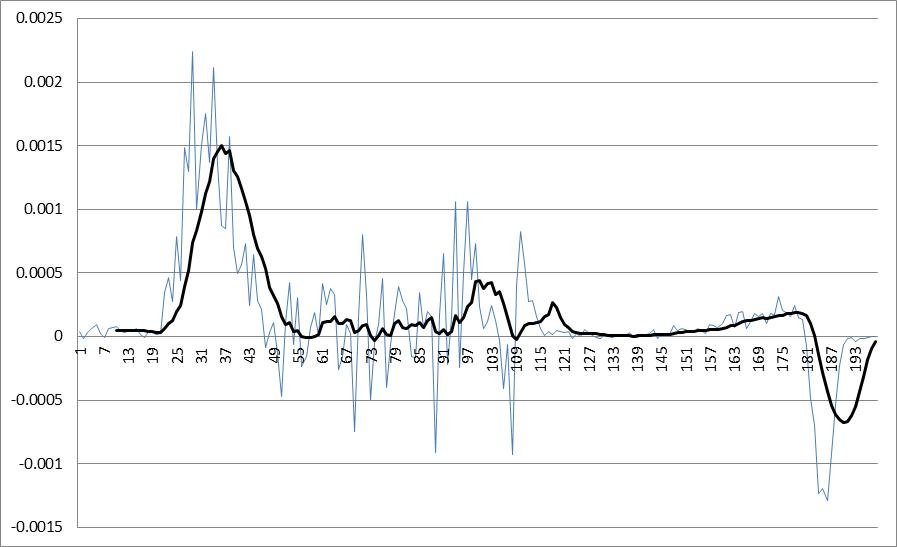
\includegraphics[width=0.5\columnwidth]{ChapterEcon/figures/exampleagglom}%
\caption{Example of agglomeration over time, measured with mean nearest neighbour distance.}%
\label{fig:agglomex}%
\end{figure}
�
This dual purpose, however, hides an effect that comes from the type of space used. The CES approach used in \gls{ge}, built on the \gls{dxs}, guarantees a diversity of firms. As will be shown in chapter \ref{chapter:models} in detail, however, space itself can provide that diversity in a two-good model where, in discrete space alone, such a limited number of goods would lead to problems. The basic issue is that several firms competing on a single point, selling the same good, find themselves in a \gls{bertcomp} situation: lowering their price by a tiny amount will result in taking the entire market, where consumers are all on the same spot. The analytic, rational result is for firms to set price at marginal cost (see e.g. \citealt{varian_intermediate_2006} p.495). In an \gls{increts} situation, however, the result will be that if one firm gets a toe-hold in cheaper production, cumulative causation leads to monopoly.
..
% little cuttinz!
%%%%%%%%%%%%%%%
Proximity is 
Glaeser is rather less equivocal about the importance of proximity: 
\begin{quote}
``The benefit of being in a city is closeness to the other people in that city... Proximity reduces transport costs for goods, for people and for ideas.'' (\citealt{glaeser_cities_2008} p.117)
\end{quote}
For Glaeser, this basic fact about proximity gives a straightforward way to define agglomeration: ``agglomeration economies exist whenever people become more productive through proximity to others'' (ibid p.5). 

\begin{quote}
``The benefit of being in a city is closeness to the other people in that city... Proximity reduces transport costs for goods, for people and for ideas.'' (\citealt{glaeser_cities_2008} p.117)
\end{quote}
For Glaeser, this basic fact about proximity gives a straightforward way to define agglomeration: ``agglomeration economies exist whenever people become more productive through proximity to others'' (ibid p.5). 

I should define agglomeration, for my model. No reason why that can't happen there. Er. Noting that it's different for discrete regions and continuous spaces. The former is a very straightforward gravity-model approach, used even by GE. The latter, I am defining as change in mean nearest neighbour distance over time. That makes it separate from agglomeration effects - which are really 1st nature effects in continuous space. (Because analytically you can't tell them from any other; e.g. backyard: one small seed of agglomeration becomes as much a 1st nature effect as a port.)
%``Urban centres came into existence because they concentrated 
% CUTTINZ
%%%%%%%%%%%%%%%

%It can be argued that many of the key distinctions in \gls{ge} flow from the maths: the clear blue water between perfect and imperfect competition models is a consequence of the maths, not of the real world. 

%Fujita, in his retrospective on Isard's `Location and Space Economy', wonders what Isard meant by the `particular effects' of space costs; he concludes Isard probably meant the impact of ``the monopolistic elements that spatial costs necessarily introduce into production theory.'' \fixref{Fujita on Isard p.376.}

%In reality, space-costs must be as much a part of the production function as any other factor. Without this fact it is impossible to explain why any firm would want to locate closer to a market, or that doing so offers that firm a real competition advantage over others. 

%As mentioned, geographical and urban economics assume different things about space. The former assumes discrete regions, each with no internal structure as such; all that matters is the interaction between regions. Agglomeration comes about through a feedback between the location choices of firms and people, whose productivity is effected by transport costs and economies of scale. A merit of this approach is its parsimony: two regions suffice to make its point, as will be discussed below. Urban economics assumes a central reference point around which spatial equilibrium results. However, both share two motivations. Firstly, to build on a foundation of individual behaviour. 

%1st vs second nature:
%This is a problem that will arise again when the nature of spatial externalities are discussed; two-dimensional, explicit categories of space can make several common GE concepts hard to sustain - yet they also offer useful ways to think about spatial organisation in the abstract, a fact not lost on some of the classical location theorists.

%No claim will be made here about the future of transport costs, but there are several reasons why it would be worthwhile not to assume their continued decline, and why that should inform abstract model-building in this thesis. Two of the most pressing are: first, fuel costs could change as oil demand outstrips supply. Such `peak oil' arguments are made very rarely in the literature at present, though they are starting to regain more credibility again, after a period where resource depletion analyses have been out in the cold. A second reason is climate change: whatever the policy outcome of current climate change negotiations, there is a likelihood that carbon will cost more in the future. It is at least worth asking, then: might there be benefits from considering the fact that costs can go up as well as down? What modelling tools exist for thinking about the likely impact of such cost structure changes? A strength of agent-based location theory, it will be argued, is that it does well at examining the impact of such changes over time. \cmt{fix cross-ref to BY model}(See model run 5.2.2.3 below.)

It would be nice if there was a clear way to separate the reality of space costs from how they are theorised. Things are messier than this, however: they cannot be boiled down simply to what can be measured. An example where measurement is a particularly thorny problem can be found in the trade cost literature; 
Trade cost cuttinz
here, the goal is trying to identify the reality of space costs. So what actually lies underneath the aggregate percentages Anderson and Wincoop have produced? It is difficult to say, since there is such a large gap between that reality and the figures, via their particular methodology.
%This would be an argument for building models to help with ontological prediction: to know what to look for. 
While Anderson and van Wincoop note that there are ``many difficulties in measuring and inferring the height of trade costs and their decomposition into economically useful components'', they do 
about spatial preferences - but doing this requires a theory to explain those choices. 
DOT drops as EU / US subcontract to Eastern Europe and S. America. [33/20] political developments, then, not changes in space costs.
cf. other political points: Whole issue is a difficult problem for abstract analysis.
European Union and U.S. Retail Gas taxes: 60 to 75 per cent and 20 to 25\% respectively.
Road tax; Motor Carrier Act etc. [23]
Should be put next to Fujita's points... where are they now?

Some types of space cost data are relatively easy to acquire, such as tariff data. Others, as Behrens points out, are so challenging that workarounds are needed (\citealt{behrens_changes_2007} p.626). 
This appears to make any approach based on simply measuring the physical cost of movement look very problematic. 
Such an approach has already meshed what objective component of space cost exists with a theory about how actors will respond to them. 
Most common method for describing space cost in aggregate: distance decay functions.  Gravity models.  Chapman 180/15.  High decay goods
Anderson and Wincoop come up with numbers describing the `tax equivalent' costs of trade for a `representative rich country': 170\%. This breaks down into ``21\% transport costs, 44\% border related trade barriers and 55\% local retail and distribution costs.'' [626]
%a place where the reliance on `empirical' answers is very model-heavy. 
They use a gravity model, though one they consider superior economically, because theoretically grounded. 
It is not an easy problem to fix. Caught between two different issues: it is possible to get data for basic transport costs - that is, the actual money cost of moving stock across space, as a proportion of overall business costs. But as the trade cost puzzle illustrates, this approach clearly misses a large chunk of space costs. 
Anderson and van Wincoop (\citeyear{anderson_trade_2004} p.692) point out, ``a theoretical approach is inevitable to infer the large proportion of trade costs that cannot be directly measured in the data''.  
Evidence shows that in many countries, distance of trade has actually been decreasing - ``distance impedes trade by 37\% more since 1990 than it did from 1870 to 1969'' (\citealt{carrere_distance_2009} p.6) This affects poorer, more distant countries much more than the main centres of economic activity. 
There is an empirical question here, overlapping with studies examining the trade cost problem: how to find out, firstly, what has actually been happening and secondly, why? Role of theory.
Accessible vs inaccessible data
Disdier and Head are one further step removed from reality, producing a meta-analysis of trade cost estimates from the literature, even attempting to correct for selection bias (\citealt{disdier_puzzling_2008}). 
Chapman imagines a world without distance, where Star Trek's teleporters are the norm: "the universal availability of the kind of technology at the disposal of the Star-trekkers would transform these [spatial] relationships by effectively nullifying the role of distance as an obstacle to movement between one place and another." [1] The impact of this obviously impossible technology is equally impossible to predict. Would all of the various mechanisms of trade costs disappear as well? Are they all dependent on the `friction' of space costs? 
..
Trade cost estimations are a good foil for thinking about the nature of total versus `accounting' costs, such as basic freight rates. 
�
Other cuttinz
%WUD 21	Common def of 'localisation' actually opposite to GE. Dispersion, move towards autarky.
%http://transitionculture.org/2010/07/30/localism-or-localisation-defining-our-terms/ Useful: so, I should be able to cite Hopkins.
As a final note for this subsection: a common meaning of the term `localisation' in the non-economic literature is actually opposite to how it is understood in \gls{ge}. Hopkins cites Shuman: ``It means becoming more self sufficient, and less dependent on imports.'' As Hopkins says, it is about ``building more localised economies''. In \gls{ge} terms, however, this is exactly the opposite: it is moving in the direction of autarky, where regions become less specialised. It is actually dispersion.
\fixref{localisation: Hopkins' dissertation}
%How would that compare with the distinction between localisation and urbanisation economies? Hmm...
�
It is not necessary to outline the full details of the model here; Brakman \emph{et al.} and Fowler are both good places to get these. Appendix \ref{apx:maths} gives an explanation of the model sufficient for getting a simulation up and running and understanding the results, and discusses some model nuts and bolts further. The task of this section is pull out those features of relevance to understanding the key space concepts. 
%Krugman's original \gls{coremodel} illustrates all the principles of \gls{ge}. This section pulls out the relevant key concepts. Section \ref{coremodelapx} of the mathematical appendix has more detail on the structure of the core model, but it is kept out of here to keep a focus on those aspects of direct interest for the thesis.


More cuttinz

That is potentially quite a confusing list, but it is important to state it explicitly, and work through the theoretical inter-relations between the terms. 

The definition of a `cost' itself, economically, needs some explanation. One of the central goals of economics is to understand the impact of \emph{all} costs. In practice, what this means is that often a mathematical description of costs will be used to discuss quite a range of real-world cost equivalents. 

%Need to x-ref forward with this, I think. And, is this the place for this discussion? It could perhaps go in the philosophy section? Which is then starting to look like a separate chapter again.

%Think I want to say here: you end up with e.g. something like density cost standing in as a proxy for several other costs - and that's OK. 
%Also cx2 2nd nature cost... 

The quantity of fuel needed to move a given distance is one of the few objective elements involved.  The total cost is a much messier proposition. 
The job of this section is to provide an overview of the reality of space costs. This is not meant as a substitute for empirical data, but instead to ward off the dangers of going too far in the direction of \emph{a priori} model-building, where `common sense' assumptions about space can easily be shown to be contradicted by the briefest of glances at empirical reality. Chapter \ref{ABM or another one?} explores in more depth how the modeller can approach this trade-off between model and real world: to pre-empt that discussion, all models must contradict reality to some extent. It is the modeller's job to be aware of where that happens, and so be able to correctly interpret the model given its particular limitations.

Regardless of how simple a model is, as full an understanding of the complexities of reality as possible will make model interpretation better. A particular target for critics of location theory has been the use of abstract Euclidean space: a featureless plane, clearly nothing like reality. One job of this section is to examine this particular assumption, and explain why it is being kept. The conclusion will then come back to this as an example of thinking about the trade-off between model simplification and a more complex reality. (Was the simplification justified? How to tell if it was justified? Noting that 'because is was easier / simpler' cannot justify it by itself...)
Chapman notes an early study by Timbers (\citeyear{timbers_route_1967}) that examined routes between 780 pairs of towns: the average route factor was 1.17. As places develop, then, networks move towards complete connectivity: 
Pose the question instead as: how do incentives of different actors interact with cost changes to produce route and infrastucture morphology? It is, first, a very important and largely unsolved problem, and, second, beyond the scope of this thesis. But it must not be forgotten when discussing the results of any model wanting to say something about space cost change in two-dimensional space.
%Is a drive for endogeneity useful? Is it the same thing as looking for generality?
%This sort of analysis is much less a part of geography now, tending instead to be grounded in the more recent physics-led resurgence in network analysis. A particularly good example of this is 
cf. Ladley... but then Wilhite above. Eek. 
Returning to Haggett's pointing out the lack of a comprehensive route model: one might argue it is simply impossible to develop such a general, endogenous model that could parallel the drive for endogeneity in other areas of economics. Gastner and Newman's work, for example, assumes given network vertices and allows the growth of edges from those, and network economics tends to consider action on fixed networks. Behrens (\citeyear{behrens_changes_2007}) take a model `case study' approach to see how a small fixed network with intervening opportunities effects a space cost change situation. 
%More interesting: what is the outcome from these tensions? Who actually drives route choice? It isn't a simple reflection of consumer demand. 
%precisely the problem: normative analyses in transport geography \emph{are} connected to reality - perhaps more than any other economic realm, transport is a matter of public policy, not merely the result of competing private interests - though of course, reality is some fiendish tangle of these.

So compare to DOT: what role route development over time, and the interests? Hugely interesting: still true now that no model exists; is that because no generalisations are possible? At any rate, biggest area that I can't do here.
%Note comparison to MAR and Jacobs externalities in that paper though... 
%May want to go back and check the WoS citations for that again, if possible: some interesting stuff. And plenty of time, eh?
�
%Button: "Time savings at work permit a greater output to be produced within a given time period which, again, drawing on the marginal productivity theory of wage determination, will be reflected in the marginal wages paid." [10/100]
�
One obvious conclusion: it is possible to have endogenous first nature effects. In an agent model, the actual location of those first nature effects will vary entirely normally as the random seed of the model is changed. Section \ref{sec:keyconcepts_coremodel} points out the importance of cumulative causation for \gls{ge}, but this somehow seems to focus too heavily on the idea that second nature effects should be isolated. In an agent-based, iterative context, that is not possible. As will be argued, there is a related problem in defining externalities over several timesteps, for actors in continous space.
%It is worth noting that, historically, `backyard' production of various sorts has been a commonplace. Sheffield cutlers, for example, worked in this way, with many homes having their own mini-forges. \cmt{Sheffield cutlers? Citation?} 
%An example used in this thesis, from the list above, is density cost: as section \ref{sec:densitycostsetup} explains, a cost based on density of actors can stand in as proxy for combined land and congestion costs. 
%As with congestion, many of these costs can often be difficult to quantify, though 
%"one between 1980 than 2000, commute times rose by about 13% for the combined 75 areas." 
% (though not impossible, see \fixref{congestioncostrefs}), but this fact does not rule out their inclusion in a modelling problem. 
G/K: "manufacturing has declined as well and now represents only 14.1\% of the economy."
This is all U.S.  What about outsourcing of production globally?  What impact on space costs?  Has there been any actual drop in weight/distance of consumed goods?
Food: Chapman.  Farmers cultivating many distant plots hedge bets.

So. Chapman [23] General findings: smaller firms less economically led; large firms, not short term profit but long-term stability and growth. Hmm.
So, larger firms always about managing risk to stay stable over time; more-so now, lean retailing etc...
The four types of space are:

\begin{enumerate}
	\item Discrete, single dimensionless point: distance does not enter into actors' considerations at all. 
	\item Discrete, $n$ points: like the core model of \gls{ge}, the simplest of which uses two discrete regions. Costs are defined between regions; internal to those regions, there are no distance-related costs (though spatial effects of being `here' may still be present; see below.)
	\item Continuous, one-dimensional: either a line or a `racetrack', which is a line with no defined start and end point that `wraps' around into a loop. A one-dimensional line or racetrack is the simplest way to define a continuous space.
	\item Continuous, two-dimensional: this can either be `wrapped' (a flat torus, locally two-dimensional) or have edges.
\end{enumerate}

  or - an example from a particular industrial sector - `basing points' for steel prices in Europe and `Pittsburgh plus' rules in the U.S (\citealt{chapman_people_1979} p.117).
Of course, the space cost of all firms' biggest input takes priority: proximity to the labour market. Labour is also the largest source of extra value input into the production process. The majority of value embodied in transported goods comes from this source, rather than the intrinsic value of the good itself. 
\fixref{any citations for labour as largest source of value?}

%This chapter examines the nature of costs - what they are, how we know about them, how many of them are theoretical structures rather than something as concrete as the cost paid at the petrol pump. See - there is a story here, if I can get it.
%As discussed in section \ref{sec:spacechange}, any factor that can be used to `buy movement' will be labelled an \gls{mbf}: units of distance can be bought with it. Depending on the type of actor, specific \gls{mbf}s \emph{must} be spent to cover distance. The most obvious \gls{mbf} is time: it takes a certain quantity of time to cover a given distance. For the sake of readability, `units of distance' will be referred to as `miles': these are entirely abstract, and are used purely to make description more readable (`miles per day' rather than `distance units per day'.) A factor can be an \gls{mbf} as well as a standard productive factor entering into a firm's production function. Again, time fits this description: where People are not putting time into moving, they can put it into production. Often, economic models use the term `labour' to refer to this productive factor; in the core model, it is the only factor. In more detail:
...
Distances will be described this way:

\begin{itemize}
%\item For each model day, each actor is given $t=1$ to spend: in other words, they have `one day per day' and will aim to make optimum use of it. (See note below for more on this.)
\item A given distance between $r$ and $s$ will be labelled $rs$. The time is takes to cover it is $t_{rs}$. So, generically, $t_{rs}=f(rs,tech)$, where $tech$ is some technology that has an impact on the time taken. For many of the models, time to cover a given distance will be a function of the distance alone. However, the generic factor $tech$ here indicates that the amount of time to cover a distance may change. 
\item $tech$'s role in this function is separate from its cost. For example, if $t{}_{rs}=rs/tech$, the time taken to travel between $r$ and $s$ goes down as the level of $tech$ increases. It says nothing about $tech$'s cost. Indeed, from the point of view of actors, it could be free and ubiquitous.
\end{itemize}
Why use the concept of time at all if it is potentially this confusing? As this section goes on to explain, if people's time is the largest determinant of their location, it needs explicit consideration. It's implementation in the model can be simplified, but if time is reduced to `just another factor' used to buy either movement or goods, it is nevertheless important to be aware of the more complex reality being glossed over.
%Yet \gls{ge}'s core model replaces this with two dimensionless points in space; Isard for one seemed to have no time for this sort of ``one point world, which somehow or other is conceived as divided into n parts, representing n nations, between which trade and trade barriers exist'' (\citealt{isard_location_1956} p.26). This thesis uses agent modelling as a novel way of unpicking the implications of the exact choice of space type.
...
Spatial agent modelling is obviously nothing new. As will be discussed in chapter \ref{chapter:ABM}, however, it appears to have largely steered away from traditional economic questions of the sort Isard and Krugman discuss: see, for instance, a recent review (\citealt{torrens_agent-based_2010}). \gls{abm} theory in the round tends to emphasise complexity over simplicity, and often defines itself against the standard canon of micro-economic ideas. This leaves a hole that agent modelling has avoided: asking the simple, `general location' questions about space that Isard - and now \gls{ge} - examine, but leveraging the particular strengths of \gls{abm}. Efforts have already been made to re-cast the central model of \gls{ge} in agent form: Christopher Fowler's work (also discussed in chapter \ref{chapter:ABM}) has the explicit goal of testing whether agent modelling can work within the constraints of \gls{ge}'s core structures. This thesis comes from the opposite direction to Fowler: it starts from an agent-oriented point of view, and points towards \gls{ge}. This leaves some very elemental questions about agent modelling of actors in space left open.
...
%Bertrand paradox; CES needed to avoid monopoly in discrete regions; not needed in 2D continuous space. MM2 50	Does R2, by default, break out of Bertrand's paradox? (Cf. Bertrand's paradox and differentiation.) Cf. 
%"Well, having just run another Torus model, I realise that space - introducing differentiation as it does - solves many of the problems inherent in point-economies, and does away with the analytic need for a product differentiation function like the CES for avoiding monopoly." (fielddiaryAutum2010 p.18)
%Oh I see: because competing in space� 
%FDA 17	Avoiding total monopoly on a point: CES and monocomp. Avoiding monopoly in the real world: 2D space. Cf. Isard on overlapping markets.
%Or p.18: continuous space - introducing differentiation as it does - solves many of the problems inherent in point-economies, and does away with the analytic need for a product differentiation function like the CES.

%WUD 44	think I need some very simple math examples for:
%http://www.kgbanswers.com/is-nix-a-word/4042728 Is nix a word? Yes!
%Though note: those inc rets could be either productive or utility / love of variety, and like the cobb douglas, they would actually look the same!)
%Also, is that true if linear output is heterogenous? E.g. comparative advantage.
\cmt{What I want to talk about here: this is another case where it might not be useful to carry on with the specifics of market stucture assumptions, i.e. drop them and see what happens. LoV in particular shows itself useful for modelling with agents, since it allows a very simple approach to trading with multiple partners in geographical space. This bit needs writing up at end.}
..
%There are two good reasons for looking at Krugman's original \gls{coremodel}. Firstly, it can serve as a useful way for understanding how space has been theorised in \gls{ge}. Later, in chapter \ref{chapter:ABM}, the work of Christopher Fowler on creating an \gls{abm} version of Krugman's model will be a useful jumping off point for explaining the approach taken in this thesis. Secondly, it presents ample opportunity for exploring how a now well-developed, but relatively new, approach has dealt with the `realism versus relevance' debate. It is particularly good for this since the issues have been openly discussed. 
...


Glaeser argues that transport costs are so low that they need not be considered in analyses: only people's time costs are worth paying attention to. This point overlaps with the `ecological criticism' discussed in section \ref{sec:ecocrit}: it seems, mathematically, that transport costs can be reduced simply by \emp{increasing} the cost of other inputs into the production process. By making other inputs more expensive, the importance of space can be lessened, with no limit on how much they can be reduced. 

A spatial version the ecological criticism might go like this: it is obviously nonsense to think that distance costs can be reduced to nearly zero simply by increasing the value of other inputs. There are hard cost limits to moving goods and people. Now, the example of the service industry suggests that the less transport costs are part of a firm's production function, the less their decisions will be determined by spatial considerations. More broadly, value density indicates the same things for goods moving within firm production networks, and on to consumers. But Glaeser's argument is clearly not that space has stopped mattering. The question seems to be: what happens in space when good costs and people costs change, relative to each other? The thesis model is set up to examine this problem.

%A world where space no longer matters is science fiction. Indeed, Chapman imagines something like that, where Star Trek's teleporters are the norm: "the universal availability of the kind of technology at the disposal of the Star-trekkers would transform these [spatial] relationships by effectively nullifying the role of distance as an obstacle to movement between one place and another." (\citealt{chapman})
The second is that time is a unique factor. It is set apart not by its relationship to production or space, but rather its source: an uninterrupted  flow is given freely to actors, at exactly the same constant rate. 
Core model cuttinz

\subsection{The core model: under the bonnet}


The \gls{coremodel} examines the interaction between a direct `transport cost' and externalities to make its case. Transport costs are defined between regions; these costs enter directly into the model's functions. In theory (see below), actors are also affected by externalities within regions: the number of workers in one region affects the total number of firms there. 

The \gls{coremodel} has two `moments' of time. The initial short run (found by a brute-force solving of a set of simultaneous equations) gives the real wage for two regions. Depending on the initial conditions, these will be higher in one region than the other. The model's second moment might be considered a second externality, as the wage level in the opposite region enters into workers' location choice. This is argued to be a natural consequence of the difference in real wages found initially: these will equilibriate as workers move region, at a rate proportional to the difference between the two regions (see \citealt{fowler_taking_2007} pp.270 for a clear outline of this.) 
%Ad hoc assumption about mobility. Highlight. Is it an advantage that mine can weigh up mobility against other costs? That dynamic needs highlighting.
%requires a separate argument. In the first, each region has its own set of simultaneous equations (See table \ref{tab:op_eqs_coremodel}) containing both regions, the real wage, the price index and regional income. 

To achieve this, the two `moments' consist firstly of a set of simultaneous equations, followed by something akin to a gravity model to do the job of finding the equilibrium level of workers. Brakman \emph{et al.} suggest there are:

\begin{quote}
``four different economic agents in the core model... namely the manufacturing workers in both regions, and the farmers in both regions. This reduces to three economic agents in the long-run equilibrium, in which the real wage is the same for all manufacturing workers.'' (\citealt{brakman_new_2009} p.128)
\end{quote}

In terms of the actual equation structure, however, the two sectors of workers are combined in one income level per region. This is a \gls{repag}, standing in for the actions of all actors in that region. (See section \ref{sec:levels} for a full discussion of this.) The migration of manufacturing workers is the heart of the model; the existence, number and location of firms is deduced from this movement. `Agricultural worker' agents have a dual purpose: to provide a positive demand for both regions (since they cannot migrate) and to act as the base of comparison for model change. They do this by providing the numeraire: agricultural output is linear, and the number of agricultural workers is fixed, so the value and quantity of this output does not change. Demand does not change for agricultural goods as other workers migrate, as they are exempted from transport costs. In effect, all agricultural produce is available from a single market across both regions, with no cost to ship them. In practice, what this means is that the number of agricultural workers can stand in as agricultural income in the final equations. (Section \ref{sec:comm_costs} talks more about the problems of translating the numeraire approach into an agent context.)

Space costs enter into the \gls{coremodel} in two ways. There is an explicit, exogenous distance cost for manufacturing goods to move between regions, and there are externalities: the discrete effect of being `here' described in section \ref{sec:extsinspace}. As well as externalities stemming from worker numbers (and thus firm numbers since, in the \gls{coremodel}, one implies the other), there is the `second moment' argument made about worker migration. While this migration can be framed as an externality, actual movement is costless - and since the location of firms is just the mirror of manufacturing workers' location, firm movement is also costless. 

One perhaps expected source of regional externality would be \gls{increts}: as workers move to a region, more input into firms means a higher average output per worker. In fact, this does not happen in the \gls{coremodel}. One parameter, $\epsilon$, stands in for several model features, including \gls{increts}, \gls{eosub} between manufacturing goods (and thus \gls{lov}), as well as the price elasticity of demand. It is set exogenously for simulation runs. Instead of a change in firm output, the regional externality manifests as a change in the equilibrium number of firms (see \citealt{brakman_new_2009} p.105.) As explained in section \ref{sec:marketstructure}, this results from the argument developed by Dixit and Stiglitz regarding `optimum product diversity'. From the point of view of utility derived from a CES function, `\gls{increts}' from an expansion in the number of varieties is still \gls{increts}.

%Actually, just need to summarise and overview of the assumption structure. Then, on...

An obvious lesson from the \gls{coremodel} is the need for a base for comparison as model values change. The \gls{coremodel} offers a useful idea: one can ask, ``what is the minimum amount of expenditure required to buy one unit of utility?'' (\citealt{brakman_new_2009} p.99) In the thesis model, `expenditure' at base is a person's time, so the question for actors becomes, `can I get more utility for my time?' This is used to help explain the model framework in section \ref{sec:howPeopleAct} - although, as section \ref{sec:agentnumbers} explains, in partial models it is just as valid to think of this quantity as simply a fixed wage.




\end{comment}


